\chapter{Theoretical frameworks and Dark Matter}
\label{BigDMtheories}
In this chapter we discuss bigger theoretical frameworks motivated by other considerations, 
that also lead to DM candidates as a side result:
theories motivated by Higgs naturalness (section~\ref{sec:Hnat}, including 
supersymmetry in section~\ref{SUSY},  composite Higgs in~\ref{sec:DMcompositeH}, extra dimensions in~\ref{sec:Xdim}, ...),
string theory (section~\ref{sec:swampDM}),
cosmology (section~\ref{sec:DMcosmo}),
the QCD $\theta$ problem and its possible axion solution (section~\ref{axion}), 
and  macroscopic objects (section~\ref{sec:MacroCompositeDMth}).
Finally, in section~\ref{sec:DMSSB} we summarise possible theoretical reasons for the stability of DM.



\section{Dark Matter and Higgs naturalness}\label{sec:Hnat}

\subsection{The Higgs mass hierarchy problem}\label{sec:hierarchyproblem}
The smallness of the SM Higgs mass $M_h=125.25 \pm 0.17$ GeV~\cite{PDG} compared to the Planck mass, $M_h\ll M_{\rm Pl}$, (or other high scales, see below) introduces a puzzle.
A calculation of one-loop quantum corrections to the Higgs mass in the SM using an explicit cutoff $\Lambda$ 
reveals quadratically divergent corrections,  $\delta M_h^2 \sim g^2 \Lambda^2$, 
where $g$ denotes the various Higgs couplings entering the loop diagrams,
such as the top Yukawa coupling and the weak gauge couplings.
While no physical effect is associated with such corrections 
(that is, all physical quantities are $\Lambda$ independent, 
and the quadratically divergent correction itself even vanishes in dimensional regularization), 
the quadratic divergence signals a potential problem. 

If the SM is augmented by new physics at a higher scale, 
such as a new heavy particle with mass 
$M_{\rm NP} \gg M_h$ and couplings $g$ to the Higgs, 
the Higgs squared mass  $M_{h}^2$ receives regularization-independent
corrections of order $\delta M_h^2 \sim g^2 M_{\rm NP}^2 \ln (E/M_{\rm NP})$,
with coefficients given by the $\beta$-functions of the theory.
Such effects are in principle measurable, and thereby physical.

The various contributions to $M_h^2$ can sum up to give the small physical Higgs mass, 
even though individual terms are much larger, of order ${\mathcal O}(M_{\rm NP}^2)$. 
Presumably there is at least one extra physical scale in the theory:
the Planck scale (around which the non-renormalizable Einstein gravity gets replaced by a more complete theory)
and possibly many others (such as the masses of extra vectors required for gauge coupling unification).
In view of this, it is surprising that $M_h$ can be so small with respect to any of these new physics scales or even the Planck mass. 
This is the so called {\em hierarchy problem}. \index{Hierarchy problem}

\smallskip

Before the start of the Large Hadron Collider (LHC) many theorists expected special types of new physics to exist around the weak scale,
such that the Higgs mass would be protected from large quantum corrections, allowing the Higgs mass to be naturally small, $\delta M_h \circa{<} M_h$.
The existence of Dark Matter reinforced these expectations, since thermal relics of
new stable particles with electroweak-scale masses and electroweak interactions 
can be a viable DM candidate, with the correct cosmological abundance (see section~\ref{sec:thermal_relic}).

\medskip

Devising theoretical frameworks where new physics at the weak scale provides a natural alternative to the SM
has been one of the main topics of theoretical particle physics (though, there have also been proposals that do not involve new physics at the weak scale, see section~\ref{sec:relaxion}).
The key motivation for these attempts was their imminent 
testability at the LHC (point~\ref{DMTsignals} on page~\pageref{DMTsignals}), which often guided the particular choices for the values of the parameters. 
After that the LHC searches yielded negative results, the research activity in this area  declined significantly. 
Therefore, we will briefly highlight the main lessons and implications for Dark Matter, rather than provide a full review.
A general theme is that the new weakly-interacting particles around the weak scale fit well with DM being a thermal relic.


\subsection{Dark Matter and supersymmetry}
\label{SUSY}
\index{DM theory!supersymmetry}
\index{Supersymmetry}
\label{sec:SUSYDM}
Among the concrete theories of natural new physics, 
weak scale supersymmetry (SUSY) has long been considered by many to be the most plausible possibility.
SUSY has several independent attractive features which go a long way toward explaining why this solution to the hierarchy problem used to be so popular. 
Below, we collect some of the main results
(for a more detailed discussion see~\cite{otherpastDMreviews,SuSyDM,SUSY:intro}).

\medskip

In what way the Poincar\'e space-time symmetry could be extended is an interesting theoretical issue,
which for a while seemed to be settled by the Coleman-Mandula theorem \cite{Coleman:Mandula}.
This theorem states that unless the new symmetries are internal (commute with Poincar\'e transformations) such theories lead to extra conserved quantities (in addition to momentum and angular momentum), forbidding scatterings among particles.
Supersymmetry is the only extension that bypasses this no-go theorem by having $N$ anti-commuting parameters $\theta_\alpha$
and thereby unavoidably linking bosons to fermions $\psi_\alpha$.

\smallskip

SUSY can be seen as a gauge symmetry that is required for a self-consistent theory of a particle with spin 3/2.
Naively,  elementary spin 1 particles $A_\mu$ contain negative-energy states, $A_0$ or $A_i$, which are, however, 
avoided by the existence of gauge symmetries.  
The self-consistency of elementary spin 2 particles $g_{\mu\nu}$ similarly requires gauging of the Poincar\'e symmetry, obtaining gravity.
The self-consistency of spin 3/2 particles $\psi_{\mu\alpha}$ (where $\mu$ is a vector index and $\alpha$ a spinor index)
similarly requires the existence of gauged supersymmetry, known as {\em supergravity}.
Gravitinos are the spin 3/2 supersymmetric partners of the graviton.


\smallskip

The SM includes chiral fermions that are compatible with having an $N=1$ supersymmetry, in which case
chiral fermions fill {\em chiral super-multiplets} that pair spin 1/2 and spin 0 particles. 
Such supersymmetric theories can also contain gauge symmetries, resulting in {\em vector super-multiplets} that pair spin 1 vector gauge bosons with spin 1/2 {\em gauginos} $\lambda$.
Chiral super-multiplets can have supersymmetric masses and interactions known as the {\em super-potential} terms.

\smallskip

A non-trivial feature of supersymmetric theories, crucial for the hierarchy problem,
 is that {\em the super-potential receives no perturbative quantum corrections}.
Technically, loop quantum corrections from scalars running in the loop cancel against similar loops with fermionic super-partners. 
However, if supersymmetry were exact, the super-partners would have the same masses as the corresponding SM particles, which is excluded experimentally. 
To be phenomenologically viable, supersymmetry needs to be broken. 
The Higgs mass remains protected from unnaturally large quantum corrections, thus solving the hierarchy problem,
if supersymmetry is broken `softly' by the supersymmetric particles receiving additional electroweak-scale mass contributions,
and thereby having weak-scale masses.

\smallskip

In the Minimal Supersymmetric Standard Model (MSSM) each SM particle is part of a super-multiplet and thus has a super-partner (these are known as {\em sparticles}).
As already mentioned above, if the sparticles have weak scale masses, the hierarchy problem is solved. Furthermore,
the RGE running of the SM gauge couplings gets modified and now allows for the SU(5) unification of the gauge couplings, at the scale
$\approx 2~10^{16}\GeV$. This is below the Planck scale and can be above the bounds imposed by the absence of proton decay, depending on the details of the model (new supersymmetric dimension-5 contributions can be problematic in general).

\smallskip


SUSY pairs the Higgs doublet $H$ with a fermionic doublet partner, the Higgsino $\tilde H$, both of which then form a super-multiplet $\hat H$.
Similarly, the lepton doublet $L$ is paired with a slepton $\tilde{L}$, forming a super-multiplet $\hat L$.
The $\hat H$ and $\hat L$ supermultiplets have the same gauge quantum numbers, which means that one can write Yukawa-like interaction terms such as $\hat L \hat Q \hat D$, which would lead to  
unsuppressed lepton-flavour violating transitions, contrary to observations (in the SM these terms are not possible since $H$ is a scalar, while $L$ is a fermion). 
To avoid this and similar problems, theorists impose
by hand a $\mathbb{Z}_2$ symmetry under which the supermultiplets housing the SM fermions are odd; thus
$\hat{L}\to - \hat{L}$, but $\hat{H}\to+ \hat{H}$. This $\mathbb{Z}_2$ symmetry can be combined with the $\mathbb{Z}_2$ under which all fermions are odd (including gauginos and higgsinos), $\psi\to -\psi$, to form the easier to remember  {\em $R$-parity} under which all the SM fields are even and super-partners odd. \index{Parity!R-parity}
Because of $R$-parity {\em the lightest super-partner (LSP) is stable and can be a DM candidate}. 
Among these, the neutralino was for a while considered to be so plausible 
that `neutralino' was often used as synonymous with `Dark Matter'. 

\smallskip

Because of a rather rigid structure of the superpotential, SUSY requires two Higgs doublets in the MSSM. In general, this would result in problematic 
charge-breaking minima and flavour violations, while in SUSY this is avoided, because it predicts 
$H_{u}$  that couples  to up quarks only, 
and $H_{d}$ that couples only to down quarks and to leptons, 
with a specific potential that avoids charge-breaking vacua.
At tree level, the MSSM predicts that the SM-like Higgs is  lighter than the $Z$ boson. 
A mildly heavier Higgs mass arises at loop level,
especially, if sparticles are much heavier than the $Z$ boson.

\medskip


The above appealing framework received a cold shower from the LHC: 
supersymmetry predicted a rich collider phenomenology, see section~\ref{sec:SUSYcolliderpheno}, 
while only the SM Higgs boson with mass $M_h = 125 \pm 0.17 \GeV$ 
was found.  
In the MSSM such a Higgs mass, significantly above the mass of the $Z$ boson, is still possible, 
but requires stops (supersymmetric partners of the top quark) to be  heavier than a few TeV.
Together with the LHC exclusion bounds on sparticles, this means that SUSY can no longer 
fully keep the Higgs mass  naturally smaller
than the other heavier new-physics scales, significantly reducing the motivation for weak scale SUSY. 
In fact, this is a problem for most of the solutions to the hierarchy problem that postulate weak scale particles (large extra dimensions, composite Higgs), 
many of which have their own DM candidates. 
In the rest of this section we review different supersymmetric particles that could potentially be DM, 
and discuss what the implications of the (so far) negative LHC results are in each case. 
The LHC will keep running to accumulate more data at the same energy $\sqrt{s}$, which will increase the sensitivity to weakly coupled states such as the DM candidates discussed below, while in other cases (such as the production of new heavy colored particle) its discovery potential has to a large extend already been exploited.





\subsubsection{Neutralino: bino DM}\index{Supersymmetry!neutralino}\index{Supersymmetry!bino}
\label{sec:Bino}
The neutral {\em bino} $\tilde B$ is the fermionic SUSY partner of the hypercharge vector boson $B_\mu$.
It mixes with the neutral component of {\em winos} (super-partners of $W_\mu^a$) and with {\em higgsinos} 
(super-partners of $H_{u,d}$), forming four mass eigenstates --- the {\em neutralinos}. 

The possibility that the lightest neutralino is mostly bino 
was often considered to be the most plausible SUSY DM candidate: 
{\em i)} various SUSY models predict this mass ordering, and {\em ii)} 
the observed DM cosmological abundance could be reproduced for a mass that matches that of natural weak scale SUSY, $M\sim M_Z$ \cite{SuSyDM}. 
Indeed, supersymmetric gauge interactions predict a Yukawa coupling between
a bino $\tilde B$, a lepton $\ell$ and a slepton $\tilde\ell$ that is
roughly equal to the hypercharge gauge coupling $g_Y$.
A tree-level exchange of a slepton with mass $M_{\tilde \ell} \sim M$ induces a $p$-wave bino DM annihilation, with a cross section
\beq \label{eq:sigmavBino}
\sigma v_{\rm rel} (\tilde B\tilde B \to \ell^+\ell^-)\sim  v_{\rm rel}^2 \frac{g_Y^4}{4\pi M^2}.
\eeq
The bino relic abundance matches the observed cosmological DM abundance for 
$ \sigma v_{\rm rel}$ in eq.\eq{sigmavcosmo}. This corresponds to
$M \sim 120\GeV$, up to order one factors that depend on the number of light sleptons 
(1, 2 or 3) and on their `chiralities' ($\tilde\ell_L$ or $\tilde\ell_R$).  

After the LHC results this simple picture faces several obstables. First of all, in SUSY models sleptons and binos are typically not much lighter than squarks and gluinos. The latter must now be heavier than $(1-2)\TeV$, given that they are charged under QCD and would otherwise 	be copiously produced in the $pp$ collisions. 
One can still consider a heavier bino
but then a larger prefactor in eq.\eq{sigmavBino} is needed in order to keep the bino annihilation
cross section at its desired value.
This can be achieved, thanks to the vast parameter space of SUSY models, but only in very specific
corners of the parameter space:
\begin{itemize}
\item[$\circ$] The cross section is resonantly enhanced for $M$ close to $M_H/2$, where $M_H$ is the mass of one of the heavy Higgses.

\item[$\circ$] The cross section gets enhanced, if some of the Yukawa couplings are larger than in the Standard Model.
This is possible in supersymmetry, since there are two Higgs doublets, $H_{u}$ and $H_{d}$,
and the ratio of two vevs, $\tan\beta \equiv \med{H_{u}}/\med{H_{d}}$, can be large.

\item[$\circ$] Bino DM annihilation can get enhanced by co-annihilations with other supersymmetric particles, for example 
stops or sleptons, if these are not much heavier than the neutralino, $\Delta M\circa{<} 100\GeV$.

\item[$\circ$] As we discuss in more details below, winos or higgsinos can be a thermal relic DM,
 if they are heavier than a TeV.
Similarly, neutralino composed of just the right amounts of bino and
wino and/or higgsino can be a thermal relic DM,  for any sub-TeV mass \cite{WellTempered}.
\end{itemize}


\subsubsection{Neutralino: pure wino DM}
\index{Supersymmetry!wino}
\label{Wino}
{\em Winos} $\tilde W^a$ are the fermionic supersymmetric partners of the $\SU(2)_L$ gauge bosons $W^a$,
with $a=\{1,2,3\}$ and hypercharge $Y=0$~\cite{Wino}.
The wino multiplet has three component,  two charged winos $\tilde W^\pm$ (fermionic supersymmetric partners of the $W^\pm$ gauge bosons)
and a neutral wino $\tilde W_3$ (partner of the $\SU(2)_L$ gauge boson $W_3$,
a linear combination of the photon and the $Z$).
After supersymmetry-breaking, all three winos, $\tilde W_{3}$ and $\tilde W^{\pm}$, receive a common mass term $M_2$.
After $\SU(2)_L$-breaking, $\tilde{W}_3$ and $\tilde{W}^\pm$
mix with the other neutral and charged fermions, respectively. 
This mass mixing is negligible in the limit $M_2 \gg v$, where 
the winos $\tilde W_3, \tilde W^\pm$ form a quasi-degenerate $\SU(2)_L$ triplet.
Only the $\SU(2)_L$ gauge interactions are then relevant for the wino DM phenomenology,
such that in this limit $\tilde W_3, \tilde W^\pm$  constitute an example of  a Minimal DM electroweak triplet with a zero hypercharge, see
the discussion in section~\ref{MDM}.
In particular, wino DM has the desired thermal relic density for $M_2\approx2.5\TeV$ (see table~\ref{tab:MDM}).
This is much larger than $v$ and beyond the reach of the LHC (section~\ref{MDM}).
The predicted direct detection scattering cross section is below the present bounds. The most stringent constraints come from indirect detection, which excludes wino DM for cuspy DM profiles of the Milky Way, while it remains valid for non-cuspy ones. 

\subsubsection{Neutralino: pure higgsino DM}\index{Supersymmetry!higgsino}
\label{Higgsino}
{\em Higgsinos} are the fermionic supersymmetric partners of the two Higgs doublets $H_{u}$ and
$H_{d}$.
Decomposing the multiplets in their components, one gets charged $\tilde{H}^\pm$
and a complex neutral Higgsino $\tilde{H}_0$ (complex, since the multiplets carry a non-zero
hypercharge $Y=\pm 1/2$).
Higgsinos can have an $\SU(2)_L$-invariant Dirac mass term $\mu$.
If $\mu$ is much larger than the $\SU(2)_L$-breaking mass terms, $\mu \gg v$,
the higgsinos form a quasi-degenerate weak multiplet of mass $\mu$.
In this limit, only the $\SU(2)_L$ gauge interactions are relevant for higgsino DM phenomenology,
such that higgsinos behave as a Minimal DM electroweak doublet with hypercharge $|Y| = 1/2$.
Higgsino DM~\cite{Higgsino:DM} has the desired thermal relic density when $ \mu \approx 1.1\TeV$ (see table~\ref{tab:MDM}).
This is larger than $v$ and beyond the reach of LHC (section~\ref{MDM}).

A pure Higgsino DM \cite{Higgsino:DM} is excluded since, due to $Y \neq 0$, it predicts direct detection scattering via tree level $Z$ boson exchanges, 
with a  cross section orders of magnitude above the present bounds, see fig.\fig{direct:typical}a.
This can be rectified by the smaller $\SU(2)_L$-breaking mass terms, leading to mass mixings with $\tilde{B}$ and $\tilde{W}_3$,
and splitting the Dirac fermion $\tilde H^0$ into two non-degenerate Majorana fermions with modified couplings.
As a result, a neutralino with a significant higgsino fraction remains excluded 
by direct detection bounds, but only up to fine-tuned `blind spots',  where different contributions to direct detection scattering
interfere negatively, allowing for tuned cancellations~\cite{WellTempered}.


\subsubsection{Sneutrino DM}\index{Supersymmetry!sneutrino}
As discussed above, $\hat L$ and $\hat H_u$ have the same gauge quantum numbers.
The lepton doublets $\hat L$ contain {\em sneutrinos} $\tilde{\nu}_L$. 
These are a possible DM candidate~\cite{Sneutrino:DM}, with the same gauge quantum numbers
as the higgsinos, but with a different spin; they are spin 0 scalars instead of spin 1/2 fermions. 
Because of this difference, the thermal relic abundance of DM is reproduced for
$ m_{\tilde{\nu}_L} \approx 0.5\TeV$, in the $\SU(2)_L$-symmetric limit (see table~\ref{tab:MDM}).
As for higgsinos, the $Z$-mediated direct detection leads to strong exclusion bounds also for sneutrino DM.
However, unlike the case of higgsino DM, the MSSM does not provide any immediate way to avoid direct detection bounds;
one needs to add, e.g., right-handed sneutrinos with a Majorana mass of the appropriate size.
Because of this, sneutrino DM attracted somewhat less interest recently.





\subsubsection{Gravitino DM}\label{sec:gravitinoDM}\index{Supersymmetry!gravitino}
The {\em gravitino} is a hypothetical neutral spin-3/2 particle; 
it is the supersymmetric partner of the graviton, predicted by local supersymmetry.
The gravitino has gravitational interactions analogous to the graviton, i.e.~couplings suppressed by inverse powers of $M_{\rm Pl}$, 
so that it can be a gravitational DM candidate~\cite{gravitinoDM}.
Its small interactions make it difficult to test it directly.

When supersymmetry is spontaneously 
broken at a scale $f$ (in a hidden sector, above the weak scale, for phenomenological reasons),
an analog of the Higgs mechanism takes place:
the gravitino $\Psi_\mu$ obtains a mass $m_{3/2} \sim f^2/M_{\rm Pl}$  by `eating' the {\em goldstino} $\chi$,
the `Goldstone boson' of spontaneously broken supersymmetry.
Hence the gravitino mass is governed by the SUSY-breaking scale, and can span a wide range of values. 
If gravity-mediation dominates all sparticle masses, all such masses are comparable.
Naturalness suggests weak scale masses, obtained for $f \approx 10^{11}\GeV$, and no specific mass ordering is predicted: the gravitino could be the heaviest sparticle or the lightest one.
Lower values of $f$ are allowed if sparticle masses receive weak-scale contributions from different dominant mechanisms (e.g.~from gauge mediation):
in such a case the gravitino is the lightest sparticle, as its mass only receives the gravity-mediated effect.
In such a case, the gravitino mass could be $m_{3/2} \sim \keV$ if $f \sim 10^6\GeV$,
or $m_{3/2} \sim\MeV$ for $f \sim 10^8\GeV$.
Gravitinos much heavier than the weak scale can arise if super-symmetry does not solve the naturalness problem.
In the `unitary' gauge the  action is written in terms of just the massive gravitino,
\begin{equation}
\Lag_\Psi=-\frac{1}{2}\varepsilon^{\mu\nu\rho\sigma}\bar{\Psi
}_{\mu}\gamma_{5}\gamma_{\nu}\partial_{\rho}\Psi_{\sigma}-\frac{m_{3/2}}
{4}\bar{\Psi}_{\mu}[\gamma^{\mu},\gamma^{\nu}]\Psi_{\nu}+\frac{\bar{\Psi}_{\mu}S_{\mathrm{vis}}^{\mu}}{2\bar
{M}_{\mathrm{Pl}}},
\end{equation}
where $S_{\mathrm{vis}}^{\mu}$ is the super-current composed of the visible sector fields.
The longitudinal components of the massive gravitino inherit the interactions of the goldstino, 
and are thus suppressed by $1/f$ rather than by $1/M_{\rm Pl}$.
Using the equivalence theorem,
the gravitino production at high energies can be approximated as the sum of two channels: the first is the production of 
a massless gravitino and the second the production of the goldstino $\chi$, where for the latter the couplings to the visible sector are given by $\bar{\chi}(\partial_{\mu}S_{\text{vis}}^{\mu})/{\sqrt{2}f}$.

If supersymmetry-breaking is transmitted to the other sparticles by interactions that are stronger than gravity --- for example through gauge interactions ---
the other sparticles will obtain larger SUSY-breaking masses than the gravitino, and thus 
the gravitino will be the lightest stable sparticle.
To be a viable DM candidate, the gravitino also needs to match the observed cosmological DM abundance. 
This can happen in multiple ways, with the main contributions usually being:
\begin{itemize}
\item[$\circ$] {\em Thermal freeze out and decay} (see section~\ref{sec:freezeoutdecay}). 
When the universe cools below the mass of the next-to-lightest supersymmetry particle (NLSP),
$m_{\rm NLSP} > m_{3/2}$,
the NLSP freezes out at its thermal relic abundance $\Omega_{\rm NLSP}$.
At a later time, the NLSP decays to a gravitino and SM particles, so that the gravitino DM abundance is given by
$  \Omega_{3/2} = \Omega_{\rm NLSP}m_{3/2}/m_{\rm NLSP}$
(for simplicity we neglect entropy production, which is a good approximation, unless the NLSP decays very slowly, while dominating the energy density of the Universe)~\cite{gravitinoCosmo2}.

\item[$\circ$]
{\em Freeze-in} (see section~\ref{Freeze-in}). Gravitinos can be produced thermally, from scatterings of the particles in the plasma~\cite{gravitinoCosmo},
such as gluon + gluon $\to$ gravitino + gluino.
The space-time density of such scatterings at temperature $T$ is given by (at leading order in the strong coupling $g_{\rm s}$),
\beq\label{eq:Buch}
 \gamma =\frac{T^6}{2\pi^3 \bar M_{\rm Pl}^2}\left(1+\frac{M_3^2}{3 m_{3/2}^2}\right)
  \frac{320.}{\pi^2} g_{\rm s}^2 \ln \frac{1.2}{g_{\rm s}},
  \eeq
where $M_3$ is the gluino mass and $g_{\rm s}$ is the SU(3) gauge coupling. 
The   second term in the parenthesis accounts for the enhanced coupling of the goldstino component of the gravitino.
In this case, the gravitino production is dominated  by the temperatures close to the reheat temperature $T_{\rm RH}$. Interestingly,
the cosmological DM abundance can be reproduced for reasonable values of the parameters:
 \beq \Omega_{3/2} h^2 =
 0.00167 \frac{m_{3/2}}{\GeV}\frac{T_{\rm RH}}{10^{10}\GeV} \frac{\gamma|_{T=T_{\rm RH}}}{T_{\rm RH}^6/\bar M_{\rm Pl}^2}. \eeq 
\end{itemize}
There are several ways that gravitino DM can be searched for. If SUSY were to be discovered at colliders and gravitino is the DM,
this could be tested by searching for the (possibly slow) decays of the NLSP 
into the gravitino (detectable as missing energy) and a SM particle
(for example, a photon, if the NLSP is the neutralino).
Gravitino DM also does not have to be absolutely stable. For instance, it is slowly decaying in SUSY models with a slightly broken $R$-parity,
resulting in indirect detection signals.
Finally, the constraints on excessive cooling of stars and supernov\ae{} sets bounds on ultra-light gravitinos~\cite{GravitinoPheno}.


\subsubsection{Axino and saxion DM}
\index{Supersymmetry!axino}
\index{Supersymmetry!saxion}
\index{Axion!saxion}
\index{Axion!axino}

The axion is a speculative light boson that provides a solution to the strong CP problem, to be discussed in section~\ref{axion}. 
To form complete chiral supermultiplets requires two additional particles: the {\em axino} $\tilde a$, which is a fermionic superpartner of the axion, and the {\em saxion}, 
$\bar a$, which is its bosonic supersymmetric partner, required in order to match the number of bosonic and fermionic degrees of freedom.
The QCD coupling of the axion super-multiplet
is the supersymmetric extension of the axion coupling to gluons, see eq.\eq{axioncouplings}. As in the non-supersymmetric case, the interactions are  
suppressed by the axion decay constant, $f_a$.
In some SUSY models, the lightest supersymmetric particle can be either the axino or the saxion, which then can constitute in principle viable DM candidates~\cite{Axino:DM}. 
The analyses  of the cosmological abundance of the axino, as well as its observability, are similar to the case of the gravitino.
For instance, in the same way as the gravitino, the axino can either be produced 
from the decays of the NLSP, giving,
\beq
 \Omega_{\tilde{a}} = m_{\tilde{a}}\Omega_{\rm NLSP}/m_{\rm NLSP},
 \eeq
or from  thermal scatterings, giving
\beq \label{eq:Omegaaxino}
\Omega_{\tilde{a}} h^2 \approx 25 g_{\rm s}^6   \ln \frac{3}{g_{\rm s}} \frac{m_{\tilde{a}}}{\GeV}
\frac{T_{\rm RH}}{10^{4}\GeV}\bigg(\frac{10^{11}\GeV}{f_a}\bigg)^2.
\eeq
Above, we chose a value of $f_a$ that is large enough such that the astrophysical bounds on axions are evaded (section~\ref{axion}). 
This then gives the correct relic abundance of GeV mass axino DM for relatively low reheat temperature, $T_{\rm RH}\sim 10\TeV$ 
(and for appropriately higher $T_{\rm RH}$, if the axino is lighter).



\subsection{Dark Matter and weak-scale extra dimensions}\label{sec:Xdim}
\index{DM theory!extra dimensions}
While weak scale supersymmetry has been considered by many as
the most plausible solution to the Higgs mass hierarchy problem, a number of alternative scenarios have also been explored.

Compact extra dimensions can provide a solution to the hierarchy problem, since gravity spreads into a volume with more dimensions. 
The large four-dimensional Planck mass is therefore only an apparent scale, experienced by a four-dimensional observer,
while the true quantum gravity scale, describing the interactions of higher dimensional gravity,
can be much lower than the 4-dimensional Planck mass~\cite{X-dim:hierarchy}. 
A tentative solution to the hierarchy problem would arise if the scale of quantum gravity could be pushed all the way down to the weak scale, 
while remaining in agreement with experimental data. 
Before the start of the LHC the constraints on these types of scenarios mostly came from indirect precision measurements, which may be evaded in special constructions. 
This rethinking of the hierarchy problem  also lead to novel attempts at constructing viable DM candidates~\cite{xdimDM}.

\medskip

The most striking experimental consequence of extra dimensions is that any SM particle 
with access to extra dimensions would be accompanied by a tower of Kaluza-Klein (KK) excitations
with mass splittings on the order of the compactification scale. 
The simplest model introduces one 5th dimension, a circle with radius $R$.
If all SM particles freely propagate in it (a situation known as the {\em universal extra dimension}~\cite{X-dim:hierarchy},
their KK excitations have masses 
\beq M_n  = n/R \eeq with integer $n\ge 1$.
Conservation of momentum in the 5th dimension becomes conservation of KK number $n$.
{\em The lightest KK modes (LKP) with $n=1$ would be stable, and could be a DM candidate}. Examples are the first KK mode of the photon
(at tree level this tends to be the lightest, so it has been considered as the most plausible candidate and is arguably the one that has received most attention), 
or the first KK modes of the $Z$ boson, the Higgs, the neutrinos or even the gravitons\footnote{See however section \ref{sec:swampland} for a different realization of the latter case.}.

This simplest model is not phenomenologically viable, since the would-be SM fermions --- the $n=0$ modes of the fermionic fields --- are not chiral.
The chiral SM fermion field content can be recovered if the extra dimension is an {\em orbifold}, i.e., 
by imposing a $\mathbb{Z}_2$ reflection symmetry on the extra dimension, 
transforming the circle into a segment with length $\pi R$.
This breaks translation invariance, and thus also breaks the KK number, but
 leaves the $(-1)^n$ $\mathbb{Z}_2$ subgroup unbroken. This so called {\em KK parity} may or may not be broken by quantum corrections (see the discussion below).\index{Parity!KK-parity} If KK parity is unbroken, 
the KK number can only change by an even number, and the lightest KK remains a stable DM candidate.

\smallskip

Taking the KK photon as an example, the total annihilation cross-section is approximately given by 
$\langle \sigma v\rangle \approx 0.3 \, g^2/\pi M^2$ \cite{xdimDM}.
The observed cosmological abundance of DM is then reproduced for $1/R \approx 0.9\TeV$~\cite{xdimDM}, 
a value comparable to the bounds from electroweak precision data~\cite{xdimDM} available before the LHC.
The collider phenomenology  resembles loosely the phenomenology of the weak scale supersymmetry:
colored KK excitations are pair produced with large QCD rates, resulting in events with jets and pairs of DM particles, which are then seen in detectors as missing energy signals.
No signatures of the extra dimension were found at the LHC. The resulting bounds on the
compactification scale, $1/R\gtrsim 2\TeV$~\cite{xdimDM}, exceed the value suggested by DM abundance,
as well as the range motivated by a natural solution to the hierarchy problem. 

\smallskip

Quantum corrections tend to generate kinetic and other interaction terms that are localized at the boundaries of the orbifold segment.
Because the theory is non-renormalizable
 (the SM gauge, Yukawa, and scalar quartic interactions are no longer renormalizable in higher dimensions),  such corrections are UV divergent.
Generic localized terms would break the KK parity.
In order to keep DM stable one needs to impose that also the terms on the borders of the orbifold segment respect the KK parity. 
Moreover,  localized boundary terms in general also modify the KK masses, preventing one from  predicting which KK excitation is the lightest and thus a possible DM candidate. 


Non-minimal extra dimensional models allow significant flexibility: beyond the choices of the field content and the symmetries, 
there is now also the possibility of choosing the extra-dimensional `geography'. 
On the flip side, this also adds a layer of arbitrariness not present in the four dimensional model building, 
rendering the constructions with stable lightest KK modes even more exceptional. 
Some KK parities are unavoidably broken by quantum anomalies, 
 whose existence is a consequence of the chirality of the fermion zero modes~\cite{xdimDMano}.
Generically speaking, more extra dimensions imply more KK modes, and thereby stronger collider constraints on their sizes.




\subsection{Dark Matter and composite Higgs}\index{DM theory!composite}\index{DM theory!technicolor}
\label{sec:DMcompositeH}
New strong interactions could be a solution to the hierarchy problem: in QCD, the low-energy scale $\Lambda_{\rm QCD} \sim$ 1 GeV is naturally small thanks to the logarithmic running of the strong constant,
and pions are parametrically lighter than this scale because they are pseudo-Goldstone bosons of a spontaneously broken approximate global symmetry, $\SU(2)_{q_L}\otimes \SU(2)_{q_R}\to \SU(2)_{q_V}$. 
Similarly, the weak scale could be naturally small, 
if the Higgs doublet is, in complete analogy with the QCD pions,
a composite bound state of fermions (termed {\em techni-quarks}), bound together by a new strong interaction 
(termed {\em techni-color}, in analogy to color~\cite{technicolor}) that confines around the weak scale.
Technicolor models can result in a composite DM candidate, where in broad terms the discussion of composite DM models in section~\ref{sec:compositeDM} still applies,
but with the additional constraint that the model  must also provide a composite Higgs at the weak scale.
This additional requirement introduces several challenges:
\begin{enumerate}
\item As indicated above, the QCD pions are mildly lighter than the $\sim1$\,GeV QCD scale because they are the pseudo-Goldstone bosons of the accidental $\SU(2)_{q_L}\otimes\SU(2)_{q_R}$
chiral symmetry in the light quark sector, $q=\{u,d\}$, which is spontaneously broken by the  $\med{\bar q q}$ condensate to its vectorial subgroup $\SU(2)_{q_V}$.
A similar $\mathcal{G}\to \mathcal{H}$ pattern of chiral symmetry breaking could have kept the Higgs mildly lighter than the new confining dynamics.
However, the measured top and Higgs masses imply that the Higgs 
has sizeable interactions with the top quark and sizeable self-interactions,
and thereby that the Higgs, apart from being light, does not exhibit the typical characteristics of a pseudo-Goldstone boson.
\begin{itemize}
\item[$\circ$] Within relatively complicated effective models the Higgs mass could still be kept naturally small,
while allowing for a sizeable self-coupling of the Higgs and a large top quark Yukawa coupling, by introducing new symmetries. A well known example is {\em little Higgs with $T$-parity} where the new symmetry, {\em $T$-parity}, may also be responsible for DM stability~\cite{littleHiggs}.\index{Parity!T-parity}
In this case, the DM candidate is the $T$-odd partner of the hypercharge gauge boson or the $T$-odd partner of the neutrino.
\end{itemize}

\item The SM Higgs has a non-trivial pattern of Yukawa couplings to the SM quarks and leptons.
It is difficult to imagine how such a structure can arise out of simple
theories that only contain new fermionic techni-quarks with techni-color gauge interactions and masses. 
This problem can be bypassed, however,  in ways that conflict with naturalness:
\begin{itemize}
\item[$\circ$] One possibility is to introduce an additional 4-fermion interaction among quarks and techni-quarks, 
which is suppressed by a new, unrelated scale.
The stringent constraints on such interactions from flavor changing transitions 
can be satisfied, if the $\beta$-function for the renormalisation group evolution (RGE) of the technicolor gauge coupling is small 
(the tongue-in-cheek terminology is that the technicolor coupling is therefore {\em walking} \cite{walking:TC}, not running).
A warped extra dimension is conjectured to provide an approximate dual picture for such a type of strong dynamics~\cite{AdS/CFT}.

\item[$\circ$] The second possibility is to add elementary techni-colored scalars with their own Yukawa couplings~\cite{CompositeHiggsDM}. 
Such models can accidentally conserve techni-baryon number, such that the lightest techni-baryon can be stable (similarly to the proton).
If neutral, they  can be a composite DM candidate, with specific couplings to the composite Higgs.
\end{itemize} 


\item The interactions of composite particles are in general described by form factors. In the 
QFT language these correspond to a series of effective operators suppressed by the compositeness scale.
Even if the new physics can be confined to the Higgs sector, dimension-6 operators such as $|H^\dagger D_\mu H|^2$
still affect the properties of the $W^\pm,Z$ bosons, which absorb 3 components of the Higgs doublet $H$ after the electroweak symmetry breaking.
Already before the start of the LHC, the precision tests of $W^\pm,Z$ bosons were disfavouring natural technicolor theories, due to overwhelming agreement with the predictions of the SM, without any signs of new strong dynamics.
\begin{itemize}
\item[$\circ$] 
Before the advent of the LHC a common approach was to shy away from explicit microscopic descriptions of compositeness, with the hope that the upcoming experimental data will shine new light on the problem. The focus was instead on effective theories that freely assumed special  $\cal{G}\to \cal{H}$ breaking patterns of the accidental symmetry, which were 
devised such that they reduced conflicts with the precision data~\cite{coset}. 
The assumed symmetry patterns could also lead to associated DM candidates \cite{DM:composite:Higgs}. 
\end{itemize}
\item Since natural composite Higgs models predict additional structure below the scale $4\pi v\sim 2\TeV$, 
while none was observed at the LHC, the research in this direction effectively stopped to a screeching halt.
Tuned models where the Higgs is composite at much higher scales remain viable,  and could, for instance, have implications for axion DM~\cite{1208.6013}.

\end{enumerate}



\subsection{Dark Matter and neutral naturalness}\label{sec:neutral:naturalness}
A possible reason for the non-observation of natural new physics at the LHC 
could be that none of the field content needed for Higgs naturalness is charged under the SM QCD. 
In such  {\em neutral naturalness} models the production of new particles at the LHC would therefore be significantly suppressed. 
New colored particles lighter than about a TeV are typically excluded, while uncolored ones can still be allowed.
Building models that satisfy such phenomenological requirements is not easy, 
because the largest coupling of the Higgs boson is to the top quark,
which is colored and interacts with gluons (supersymmetry cancels the effects of the top quark on the Higgs mass by adding colored stops and gluinos).


An attempt in this direction are the {\em Twin Higgs} models in which the SM is accompanied by its mirror (possibly only partial) copy,
such that the mirror $\SU(3)_c$ is not the ordinary QCD gauge group~\cite{Neutral:naturalness}.
A discrete $\mathbb{Z}_2$ symmetry that exchanges the two sectors could protect the Higgs mass against leading radiative corrections, 
if it is a remnant of a larger spontaneously broken global symmetry, with the SM Higgs the pseudo-Goldstone boson whose potential, including the mass, is then tightly constrained due to the presence of the $\mathbb{Z}_2$ symmetry~\cite{Neutral:naturalness}. 
However, no such symmetry is present in the spectrum of observed particles, implying that the $\mathbb{Z}_2$ is broken. 
The protection of the Higgs mass against radiative corrections is thus only partial, and additional structure is required at energies above $\sim 10$\,TeV. 

Much like the SM the (partial) mirror copy also possesses accidental symmetries: the mirror lepton number $L'$, and the mirror baryon number $B'$, as well as the conserved  mirror charge $Q'$ 
(the mirror $\U(1)'_{\rm em}$ may or may not be gauged, though). 
These conserved quantum numbers ensure the stability of the lightest set of particles in the mirror copy, the lightest lepton $\ell'$ and the lightest mirror baryon, 
which can then be the DM candidates. 
Depending on the details, the DM can be a weakly interacting thermal relic (discussed in section~\ref{sec:WIMPs})
or asymmetric DM (sections~\ref{sec:asymmetricDM} and~\ref{sec:AsymmetricDMth}).
The latter possibility needs that the cosmological evolution resulted in an asymmetry in the population of DM particles in the mirror sector. 
If $\U(1)'_{\rm em}$ is gauged the Twin Higgs DM particles can also form dark atoms, which then has additional observational consequences (see section~\ref{sec:dark:atoms} for a general discussion). 




\subsection{Dark Matter and the relaxion} \label{sec:relaxion}
A number of different authors have proposed models in which the smallness of the squared Higgs mass is tied to the cosmological evolution.
The general idea is that the point at which the squared Higgs mass in the Lagrangian becomes zero constitutes a critical threshold that separates qualitatively different physical situations. 
When the squared Higgs mass becomes negative, this results in a nonzero Higgs vacuum expectation value, $v$, 
which then induces nonzero
masses for the SM fermions and the $W^\pm$, $Z$ gauge bosons. 
If one assumes that the squared Higgs mass is dynamically controlled by the vacuum expectation value of a new scalar singlet $\phi$, 
 the  cosmological evolution may dynamically select a small but non-vanishing value of $v$.

\smallskip

The first proposal along these lines  is the so-called {\em relaxion}~\cite{relaxion}. During inflation,
the hypothetical relaxion scalar field $\phi$ is assumed to roll down its potential, while being coupled to the Higgs via a term $\sim g  \phi |H|^2$. 
Because of this coupling the Higgs mass term evolves during the rolling phase: initially it is large and positive, while later it becomes small and negative, triggering the nonzero Higgs vacuum expectation value. 
Assuming that the relaxion has an axion-like coupling to gluons $\sim a G_{\mu\nu}\tilde{G}^{\mu\nu}/f$
($f$ is the equivalent of the axion decay constant, see section \ref{AxionInteractions}), then as soon as the SM quarks obtain the mass 
 from the Higgs mechanism,
the relaxion potential would receive a new periodic contribution $\sim \Lambda_{\rm QCD}^3 h \cos(\phi/f)$, typical of axion models (in phenomenologically viable version of the model a new group and new fermions are required not to be excluded experimentally).
This oscillatory term generates, in the rolling slope of $\phi$, grooves whose depths increase as the rolling of $\phi$ proceeds, and eventually become valleys deep enough that the field $\phi$ gets stuck at one of the local minima. This halts the cosmological evolution of the relaxion field precisely at the point at which the squared mass term of the Higgs multiplet starts having a small negative value, thereby explaining the smallness of the weak scale.

While the mechanism works in principle, it also has some less appealing features.
To make the idea viable the relaxion cannot be the QCD axion. Instead, a new confining sector and extra fermions are needed.
The coupling $g$ needs to be extremely small, and thereby the relaxion field needs to be very light, spanning a large super-Planckian  range of field values.
The weak scale is naturally smaller than the cut-off of the relaxion theory, which, however, turns out to be much smaller than the Planck scale.


\smallskip

Various subsequent variants of the relaxion mechanism tried to  improve the basic set-up. Here, we focus only on aspects relevant to DM.
In the basic scenario, the relic relaxion particles cannot be the DM, since the relaxion mechanism occurs during the inflationary period, which then dilutes the relaxion abundance. 
Variants of the mechanism, in which relaxion could be the DM, have, however, also been explored~\cite{relaxion}. 
One possibility, for instance, is that the relaxion DM is produced after reheating via the scatterings of SM particles in the plasma. This leads to DM in the keV range. 
Another possibility is that a high reheating temperature erases the trapping valleys, re-starting the rolling of the relaxion: when the temperature eventually decreases and the valleys reappear, another epoch of particle production occurs, creating the needed DM abundance (requiring that the relaxion is re-trapped in a close-by minimum guarantees that the Higgs mass does not significantly change after reheating). This leads to DM in the sub-eV range, with a phenomenology that resembles that of the axions (see section~\ref{AxionExp}).

\smallskip

A different scenario attempting a cosmological anthropic solution to the hierarchy problem and predicting an ultra-light DM candidate is the so called {\em sliding naturalness}~\cite{relaxion}.
In these models anthropic selection results in a light Higgs, because a too large Higgs vacuum expectation value triggers an instability in a different light scalar, such that it rolls down its potential, and makes
the cosmological constant big and negative, until it crunches the universe.






\section{Dark Matter and cosmology}\label{sec:DMcosmo}
\subsection{Dark Matter and Dark Energy: Chaplygin gas}
\index{Ultra-light DM}\index{DM!as ultra-light}\index{Chaplygin gas}\index{DM theory!Chaplygin gas}\index{DE-DM interaction}

At present, roughly 70\% of the energy budget of the Universe is due to Dark Energy (DE), see eq.~\eqref{eq:Omegas} in appendix \ref{app:Cosmology}. 
The question why  this energy density is so small, $V \sim \meV^4 \sim 10^{-120}M_{\rm Pl}^4$, is the so called {\em cosmological constant naturalness problem}. 
Numerically, it is even more severe than the Higgs mass hierarchy problem that we discussed in the previous section. 
Tentative natural solutions often involve new ultra-light scalars, which could be DM candidates,
but also face serious theoretical obstacles as discussed in~\cite{Cosmological.constant}.


A concrete such attempt of unifying 
DM and DE is the so called {\em Chaplygin gas model of cosmology}~\cite{Chaplygin}.
At the level of the effective description, a Chaplygin gas is defined to be a fluid that has the following equation of state 
\beq \label{eq:Chaplygin}
\wp=-V^2/\rho.\eeq
The energy conservation equation $dU=-\wp \, d{\cal V}$,  i.e., \ $d\rho/da=-3(\rho+\wp)/a$
is solved by $\rho =\sqrt{V^2+B/a^6}$ where $B$ is an integration constant.
The energy density of a homogeneous Chaplygin gas therefore initially scales as Dark Matter, $\rho\propto 1/a^3$, 
while at later times it behaves as a cosmological constant, $\rho\simeq V$.
The observed current Dark Energy is reproduced by choosing a very small $V \sim 10^{-120} M_{\rm Pl}^4$.

In the intermediate regime, $\rho$ differs from the $\Lambda$CDM model.
This regime is tested by precise cosmological observations:
the Chaplygin gas model of cosmology is excluded because its
adiabatic sound speed $v_s^2 = \partial \wp/\partial \rho$ 
is not small enough to behave as DM during structure formation,
as primordial inhomogeneities $\delta_k$ evolve as $\ddot \delta_k =-(k v_s/a)^2\delta_k+\cdots$ (see section \ref{sec:linear:inhom})~\cite{Chaplygin}.
CMB and LSS data demands $v_s^2 \lesssim 10^{-5}$, excluding $v_s^2 \sim 1$~\cite{DMsoundspeed}.

\medskip

The exclusion can be avoided by assuming a `{\em generalized Chaplygin gas}'
with equation of state 
\beq \wp = -V^{1+\alpha}/\rho^\alpha,  \eeq 
such that $\rho =[V^{1+\alpha} + B/a^{3(1+\alpha)}]^{1/(1+\alpha)}$ 
still interpolates between DM and DE~\cite{Chaplygin}.
In the limit $\alpha \to 0$ this reduces to a combination of DM and DE, as in $\Lambda$CDM,
so that the exclusion bounds are satisfied for small enough $\alpha\lesssim 0.2$. 
Of course, the Chaplygin gas model, as well as any unified DM/DE model which behaves at late times as pure DE, faces the difficulty of explaining the small scale (galactic and cluster) effects attributed to DM. For an attempt to address this difficulty, see e.g.~\arxivref{astro-ph/0601274}{Arbey (2006)} in~\cite{Chaplygin} and references therein.

\medskip

At the fundamental level, a Chaplygin gas can arise from a {\em `branon'}
---  a scalar $\varphi$ motivated by string theory, which parametrises the position of a brane in an extra dimension ---
with kinetic action of the Born-Infeld type
\beq 
\label{eq:LBorn-Infeld}
\Lag =- V \sqrt{1- \frac{(\partial_\mu  \varphi)^2}{M^4}} .
\eeq
Thanks to the higher-dimensional covariance, this action unifies the kinetic and potential energy into a Lorentz-like factor.
In the homogeneous limit $\varphi(t)$ the corresponding Hamiltonian energy density is  $\rho = V/\sqrt{1-\dot\varphi^2/M^4}$, 
and the pressure is $\wp=\Lag$, giving the equation of state in eq.\eq{Chaplygin}.
The generalized Chaplygin gas  could similarly be derived from a less motivated  action
\beq 
\label{eq:LBorn-Infeldgen}
\Lag = - V  \left[1-  \left(\frac{(\partial _\mu \varphi)^2}{M^4}\right)^{(1+\alpha)/2\alpha} \right]^{\alpha/(1+\alpha)} \simeq \frac{V}{M^4} \frac{(\partial_\mu \varphi)^2}{2}  - V +\cdots.
\eeq
For $\alpha\to 0$ this reduces to the case of having a sum of vacuum energy and DM contributions, as in the right-hand side of eq.~\eqref{eq:LBorn-Infeldgen}, 
since then the additional terms become negligible.
See~\cite{RollingScalars} for related attempts at getting DM and dark energy from rolling scalars. 


\smallskip


More general interactions between DM and dark energy are discussed in section~\ref{sec:DESIanomaly}.


\subsection{Dark Matter and inflation}
\label{sec:DMandInflation}
\index{Inflation}
Ignoring the cosmological constant problem for the moment, the $\Lambda$CDM model of cosmology still appears to require two extensions to the Standard Model: DM and inflation.
Could the two have the same microscopic origin? In fact, microscopic theories that combine the two are rather easy to write down, 
but unfortunately also tend to not give any new easily observable consequences~\cite{DMasInflaton}.

As a simple example let us take the scalar singlet DM model of section~\ref{ScalarSinglet}, where a scalar singlet DM candidate $S$ is added to the SM, but now let us require for $S$ to also act as the inflaton. This is possible,  if $S$ has a non-minimal coupling to gravity, $\xi_S S^2 R/2$.
Together with the quartic potential for $S$ in eq.~\eqref{eq:LScalarSinglet}, it is then possible to satisfy the conditions for slow roll inflation.
At low energies, the theory remains invariant under the $S\to - S$ symmetry, even in the presence of a nonzero $\xi_S$ coupling, so that 
 $S$ particles are stable and can act as DM.
During inflation, however, this symmetry plays no role, and is broken by $\langle S\rangle \neq 0$.
It gets restored once the period of inflaton ends and $S$ reaches the minimum at $S=0$.
After the end of inflation the system thermalises, resulting in a thermal bath that contains both the SM particles and DM particles. 
The stable $S$ particles later undergo thermal freeze-out, i.e., they
behave exactly as in the singlet DM model of section~\ref{ScalarSinglet}.

Going beyond the minimal version of the scalar singlet model, 
one can change what the acceptable values for the parameters of the model are. 
For instance, if DM is produced via an alternative mechanism, such as the freeze-in (see section \ref{Freeze-in}), then larger $S$ masses can also lead to acceptable DM abundance~\cite{DMasInflaton}.

More involved models have also been considered, such as in Ballesteros et al.~(2017, 2019) \cite{DMasInflaton}, which features, 
among other ingredients, a complex scalar field whose components play the role of the inflaton and of axion DM.






\section{Dark Matter and string theory?}\label{sec:swampDM}\index{DM theory!strings}


Einstein gravity is non-renormalizable and becomes strongly coupled at energies around the Planck scale.
String theory is a possible extension of QFT that brings quantum gravity under control.
However, a self-consistent description of strings as the quantum theory of gravity employs super-symmetry and 6 extra dimensions
(or possibly 7: the string theory itself could be a limit of a deeper unknown theory).
The extra dimensions should not be observable at energies we have probed so far; they need to be compactified 
in order to obtain the effectively $3+1$ dimensional space-time that we observe at energies well below the string scale.
The resulting effective QFT, characterized by the choice of the gauge group, matter content, and values of the couplings,
depends on the shape and geography of the compactification. 
Neither of these is known, either theoretically or experimentally,
with an  exponentially vast number of viable options,
sometimes estimated as $10^P$ with $P$ comparable to the number of pages in this review.

Because of the abundance of choices, extracting any definitive predictions is exceedingly difficult, if not nearly impossible.
 The existence of a vast  {\bf landscape} of different vacua may, however, change our perspective on the two hierarchy problems discussed above.
 It allows to interpret the apparent unnaturalness of
the vacuum energy and of the Higgs mass as being the results of {\bf anthropic selection} within a multiverse, populated through cosmological inflation~\cite{anthropic}.
If taken seriously, this alternative then reduces the theoretical motivation for the natural solutions to the hierarchy problems discussed in the previous sections:
maybe the value of the cosmological constant and the mass of the Higgs are simply unnaturally small and building theories of new natural physics at the weak scale is a misguided effort. 



On the other hand, extracting testable implications for Dark Matter (or for any concrete structure of the effective QFT) from theories with a large landscape of vacua, such as the string theory, is rather difficult. 


An important issue is whether the existence of  a DM abundance, that should be comparable to the observed one,
is an anthropic necessity~\cite{DManthopicabundance}. 
As discussed in section~\ref{sec:evidencesmaxi}, in the cosmological evolution of our Universe DM facilitated the formation of large scale structures and the galaxies, since it started to cluster after the time of matter/radiation equality.
At that time, normal matter could not cluster, since it was still coupled  via the $e$ and $p$ charges to photons, which cannot cluster since they are relativistic.
In our Universe, matter later fell into the  inhomogeneities formed by the DM.
Without DM, the ordinary baryons would have started clustering only after decoupling.
Since the decoupling occurred not too long after the matter/radiation equality (see fig.\fig{Omegas}), 
the extra damping would have only moderately suppressed the matter power spectrum $P(k) = 2\pi^2\delta_k^2/ k^3 $. However, this change may have been enough to have had severe consequences. 
The bottom-right panel in fig.\fig{CMBLSS} shows that the matter inhomogeneity $\delta_k$ would have remained somewhat below 1, 
thus suppressing galaxy formation and thereby the existence of `life'. 


Whether this implies that a DM abundance somewhat larger than the ordinary matter density is an anthropic necessity, is debatable. 
A fly in the ointment is that varying other parameters allows one to recover a universe with abundant structures. For instance,
a universe without any DM, but with larger primordial inhomogeneities, $\delta \approx 10^{-4}$, would have reached $\delta_k\sim 1$, just as in our Universe. 
One can also contemplate a universe with (much) more DM than measured: for a fixed value of $\delta$, having more DM relative to normal matter than in our Universe would have allowed for a bigger value of vacuum energy, $V \lesssim \delta^3 (M Y_{\rm DM})^4$, and still be compatible with formation of structure.
The anthropic constraints on universes with large DM densities are, in fact, quite loose. 
While a higher DM density would have precluded the cooling of galaxies, disk fragmentation and formation of stars, and hence `life', 
 this would occur only for values of DM density that are several orders of magnitude above the observed one~\cite{DManthopicabundance}. 
\index{DM theory!anthropic principle}

Below we describe a few more concrete attempts at deriving DM implications from string theory: the possible existence of moduli and the axiverse, string-motivated supersymmetry, and the swampland program. Let us also mention here the {\em asymptotically safe gravity} framework, in which one insists on achieving a fixed point with gravity in the far UV. The coupling with gravity can place constraints on the couplings in the dark matter model, so that some phenomenologically viable models are ruled out and others have a reduced parameter space \cite{asymptoticallysafegravity}.




\subsection{Dark Matter and string moduli}\index{Supersymmetry!moduli}
Supersymmetric string compactifications often feature {\em moduli}, chiral super-fields that either have no super-potential or have a super-potential that is negligible.
Supersymmetry forbids perturbative quantum corrections to the super-potential, therefore moduli persist also at the quantum level.
The  vacuum expectation values of the moduli are not predicted by the string theory, while, importantly, they do control the values of some of the couplings in the effective QFT, that is valid at low energies.
When supersymmetry is broken at low energies, the moduli tend to acquire masses $m$ that are comparable to the supersymmetry breaking scale.
The moduli decay gravitationally, with the decay rate $\Gamma \sim m^3/M_{\rm Pl}^2$.
Since the decay rate decreases with $m$, a modulus that were light enough could thus provide a (metastable) candidate for a gravitational DM, section~\ref{GravDM}.

This does not work in practice, however, since supersymmetry must be broken above the weak scale.
Had supersymmetry been broken around the weak scale,  $m \sim M_Z$, the moduli would have affected cosmology in a problematic way:
they behave as matter, with $\rho\propto 1/a^3$, and would have eventually dominated the energy abundance (see section~\ref{sec:misalignement}). Once they decayed they would have reheated the universe, but only
up to a temperature $T_{\rm RH} \sim (\Gamma M_{\rm Pl})^{1/2} \lesssim \MeV$, for  $m \lesssim 50\TeV$, which
is not high enough to be compatible with the BBN bounds. 
The moduli problem is avoided, if supersymmetry is broken sufficiently above the weak scale 
(in which case it is not a solution to the Higgs naturalness problem).
In this scenario, the moduli decays could contribute to DM production~\cite{moduli}.
A related possibility is that the SM vacuum could arise from a compactification that breaks supersymmetry already at the string scale.
Computational difficulties prevent studying such compactifications, that likely do not feature light moduli.


\subsection{Dark Matter and heavy-scale (or split) supersymmetry}\index{Supersymmetry!split}\index{DM theory!supersymmetry}
Since string theory appears to require super-symmetry, it is interesting to entertain the possibility that 
super-symmetry exists, but does not solve the Higgs hierarchy problem, so that 
the scale of supersymmetry breaking need not  be around the weak scale.
Furthermore, this no longer needs  to be a unique scale: the spectrum of super-symmetric partners might be {\em split} into 
two sets with very different masses,  the supersymmetric scalars at mass scale $\tilde{m}$, and  
the supersymmetric fermions at mass scale $\tilde{M}$.
Different arguments lead to different guesses for the possible values of $\tilde m$ and $\tilde M$:
\begin{itemize}

\item[$\circ$] The SU(5) gauge unification favours $\tilde{M}\sim 10^6\GeV$~\cite{HeavySUSY}.

\item[$\circ$] Within the MSSM, the measured Higgs mass can be reproduced for super-symmetry lighter than $\tilde{m}\circa{<} 10^{10}\GeV$,
although $\tilde{m}\sim\tilde{M}\sim M_{\rm Pl}$ is allowed within $3\sigma$ uncertainties~\cite{HeavySUSY}.

\item[$\circ$] Symmetries allow $\tilde{M}\ll \tilde{m}$, and a one-loop splitting $\tilde{M} \sim \alpha \tilde{m}/4\pi$ arises in some models~\cite{HeavySUSY}.

\item[$\circ$] Split supersymmetry allows DM as a weak doublet or triplet,
with DM abundance reproduced thermally for $\tilde{M}\sim \TeV$ (see section~\ref{MDM}).
Such a case is appealing, as the Higgs mass can be reproduced for $\tilde{m}\circa{<}10^8\GeV$,
and SU(5) gauge unification can be achieved~\cite{HeavySUSY}.
However, other cases are also possible, such as gravitino DM.

\item[$\circ$] Finally, a simple possibility is that the super-string landscape is statistically dominated by vacua with super-symmetry broken already around the Planck scale.
This would correspond to $\tilde{m}\sim M\sim M_{\rm Pl}$.  
\end{itemize}



\subsection{Dark Matter and the string swampland}\label{sec:swampland}\index{DM theory!extra dimensions}
Attempts of obtaining observable implications from string theory recently shifted to the so called {\em `swampland'} program:
the hope that compatibility with string theory restricts in interesting ways the 
QFTs that describe physics below the string scale.
Theories outside the string-theory landscape are said to be in the swampland.
While there is no proof of  resulting restrictions on QFTs, various conjectures have been proposed:
\begin{enumerate}
\item Gravity must be weaker than gauge interactions: particles with gauge charge $q$ must be heavier than $m \gtrsim q M_{\rm Pl}$,
such that extremal black holes with mass $M = Q M_{\rm Pl}$ and charge $Q$
evaporate~\cite{SwamplandDM}.
This would mean that a class of DM candidates, the Planck-scale remnants of primordial black holes (see section \ref{sec:PBHs}), 
are incompatible with string theory.

\item The Planck scale limits the range of scalar field values. Otherwise, the QFT description is invalidated by the appearance of a tower of
extra  states  that are light, if there are super-Planckian scalar field value variations~\cite{SwamplandDM}. 

\item Achieving the small measured vacuum energy 
$V\sim {\rm meV}^4\sim 10^{-120}M_{\rm Pl}^4$ implies a large variation of some field~\cite{SwamplandDM}.
It is however not clear what  forbids the alternative possibility that the small $V$ arises as an accidentally tuned cancellation 
between large contributions, without needing any large field range. 
\end{enumerate}
Trusting the last two conjectures and combining them, it was conjectured that the implied light tower 
can only be the Kaluza-Klein modes of one gravitational extra dimension 
with size set by the vacuum energy, $R\sim V^{-1/4}\sim 1/T_0\sim \mu{\rm m}$
(with some generosity in numerical factors)~\cite{SwamplandDM}.
This conjectured string theory prediction gives a theory of DM: 
graviton KK modes  cosmologically produced by UV-dominated gravitational freeze-in.
The space-time density of scatterings that produce one KK graviton with mass $M$ from the SM plasma
is $\gamma \sim T^6 e^{-M/T}/M_{\rm Pl}^2$.
Summing over the number of accessible KK modes $\sim T_{\rm RH} R$,
and taking into account that their typical mass is $M \sim T_{\rm RH}$
gives the DM abundance
\beq 
\label{eq:KKgravitational:freeze-in}
\Omega_{\rm DM} \sim \frac{M}{T_0} 
\left.\frac{\gamma}{H s}\right|_{T =T_{\rm RH}}  \sim  \frac{T_{\rm RH}^3}{M_{\rm Pl} T_0^2}.
\eeq
The amount of gravitationally produced  graviton KK can match the DM abundance
assuming a low reheating temperature  $T_{\rm RH} \sim\GeV$.
However, the decay rate of GeV-scale KK gravitons into SM particles
$\Gamma({\rm KK}\to \gamma\gamma, e^-e^+)\sim M^3/M_{\rm Pl}^2$ 
exceeds the bounds in fig.\fig{IDconstraintsdecay} by about 12 orders of magnitude.
To avoid being excluded one can assume mildly broken translational invariance in the extra dimension, 
such that the produced GeV-scale graviton KK
decay dominantly to lighter graviton KK with masses $M \sim 10\keV$,
heavy enough to satisfy bounds on warm DM, and light enough to be satisfy DM stability bounds~\cite{SwamplandDM}.

Furthermore, the black holes in $5$ dimensions can be alternative DM candidates, even if they are lighter than $10^{-15}\,M_\odot$
(unlike in fig.\fig{machos}b), since they emit less Hawking radiation~\cite{SwamplandDM}.


\subsection{Dark Matter and string axiverse}\label{sec:stringaxiverse}\index{Axion!axiverse}
Compactifications of the extra dimensions in string theory tend to predict the existence of very light pseudo-scalar fields that, from the low energy perspective, behave as axion-like particles
(see section~\ref{axion}).
In string theory these are the $n=0$ massless KK modes of antisymmetric tensor fields, 
with masses protected by the higher dimensional gauge symmetry to all orders in perturbation theory, while nonzero contributions to their masses do arise from non-perturbative phenomena (in a similar way as for the QCD axion, see section~\ref{AxionInteractions}). 
However, unlike the QCD axion, which is usually assumed to be just a single light pseudo-Nambu-Goldstone boson, 
the generic expectation from the string theory is that there are many such light pseudo-scalar fields, possibly even populating each decade of mass all the way down to the Hubble scale of $m_a\sim 10^{-33}$\,eV, a hypothesis that is often referred to as the {\em string axiverse}~\cite{axiverse}. 
Depending on the details of the string axiverse DM could then be composed from one or several different axions with differing masses 
(unlike the discussion in the next section, where for the most part we will assume that there is a single axion). 



\section{Axion Dark Matter}
\label{axion}
\index{Axion}\index{DM theory!axion}
The axion is a hypothetical light pseudo-scalar postulated in 1977 in order to explain dynamically why the CP violation
in strong interactions is very small (see section~\ref{AxionQCD} below).
Interestingly, the axion can be a viable ultra-light  DM candidate (section~\ref{LightBosonDM}),
possibly produced via the misalignment mechanism (section~\ref{sec:misalignement}). This section provides further details specific to axion DM.
Importantly, axion DM can be probed via its effective interactions, which are discussed in section~\ref{AxionInteractions}.
The main classes of renormalizable axion models are summarized in section~\ref{AxionModels}, while
in section~\ref{AxionCosmo} we discuss the expected cosmological relic density of axions.
In section~\ref{AxionExp} we summarize experimental efforts for detecting axion DM.





\subsection{The QCD $\theta$ angle and the chiral anomaly}\label{AxionQCD}
This topic involves aspects of advanced quantum field theory
that cannot be presented in a simple way: chiral anomalies and
extended field configurations with topological charges.
We thereby just state the main results, see~\cite{axionmodels,axionreviews} for additional extensive discussions.

The symmetries and field content of the SM allow for 
one extra CP-violating term in the SM Lagrangian, parameterized by a constant $\theta$,
\beq 
\label{eq:Lag:theta}
\Lag = \Lag_{\rm SM} - \theta\frac{g_{\rm s}^2}{32\pi^2}
G_{\mu\nu}^a \tilde G_{\mu\nu}^a,
 \eeq
where $g_{\rm s}$ is the QCD gauge coupling,
$G^a_{\mu\nu}$ is the gluon field strength and
$\tilde G^a_{\mu\nu} \equiv \frac{1}{2}\epsilon_{\mu\nu\alpha\beta}G^a_{\alpha \beta}$ its dual.
Naively, this extra term is irrelevant since it is a total derivative:\footnote{In a more geometrical language, 
the $\theta$ term in eq.~\eqref{eq:Lag:theta} can also be written as
$F=\epsilon^{\mu\nu\rho\sigma} F_{\mu\nu\rho\sigma}$,
where $F_{\mu\nu\rho\sigma} = \partial_{[\mu} C_{\nu\rho\sigma]}$
is the 4-form that follows from the Chern-Simons 3-form $C_{\nu\rho\sigma}$.
This can be seen as a QCD composite, where the QCD gauge invariance also
induces a 3-form gauge invariance on $C$.
The discussion about the role of the QCD axion in solving the strong CP problem can then be rephrased, in a more abstract language,
by noticing that a 3-form in 3+1 dimensions is analogous to a 1-form (a vector) in 1+1 dimensions;
the equations of motion are solved by a constant $F$, which is the 1+1 dimensional analog of the electric field. In the same way as a Higgsed electric field in 1+1 dimension is screened, the axion screens the 3-form by putting it in its Higgs phase.} 
\beq G^a_{\mu\nu}\tilde{G}^a_{\mu\nu}=\partial_\mu K^\mu\qquad\hbox{with}\qquad
K^\mu = \epsilon^{\mu\alpha\beta \gamma}C_{\alpha\beta\gamma},\qquad
C_{\alpha\beta\gamma}= A^a_\alpha G^a_{\beta\gamma} - g_{\rm s} f^{abc}
A^a_\alpha A^b_\beta A^c_\gamma/3.\eeq
Using Gauss's theorem such a total derivative  term in the action can be rewritten 
 as a boundary contribution at Euclidean infinity. Were $K^\mu$ to vanish sufficiently quickly at infinity, the term could be dropped. However, this is not the case for all gauge configurations in a non-abelian gauge group such as QCD. Instead, it is equal to 
the Cartan-Mauer topological invariant of the mapping $g(\hat x_\mu)$, which maps $\hat x_\mu$ parametrising the boundary (i.e., the $x^\mu$, but at Euclidean infinity, and therefore just a direction) into an element  $g$ of the SU(3) gauge group.
As a topological quantity it is quantized, and given by
\beq 
\frac{g_{\rm s}^2}{32\pi^2} \int d^4x ~ G_{\mu\nu}^a \tilde G_{\mu\nu}^a = q,
\eeq
where $q=\{0, \pm1, \pm2,\ldots\}$
counts how many times the hypersphere at infinity wraps around the group manifold (this wrapping has an orientation, and thus $q$ can be either negative or positive).
An `instanton' field configuration corresponds to $q=1$, and is given by
\beq
 G_\mu^aT^a  = ig_{\rm s} \frac{r^2}{r^2 +R^2}  g^{-1}(x) \partial_\mu g(x),
\qquad
g(x) = \frac{x_4 + 2 i x_i \sigma_i}{r},
\eeq
where $R$ is a constant controlling the size of the instanton, and $\sigma_i$ are the Pauli matrices of the SU(2) subgroup of SU(3). 
For $r\to\infty$ this field configuration is a pure gauge.

\smallskip

Such field configurations give non-perturbative corrections to the action, though
exponentially suppressed by a factor $e^{-8|q|\pi^2/g_{\rm s}^2}$. 
They are important in the case of QCD, since the gauge coupling $g_{\rm s}$
becomes non-perturbatively large for energies around the QCD scale, $\Lambda_{\rm QCD} \approx 250\MeV$.

\medskip

The QCD $\theta$ term is connected to the chiral anomaly.
The SM Yukawa couplings $y$, which lead to quark masses after electroweak symmetry breaking are, in Weyl notation, given by,
\beq \Lag \supset 
  y_U\,  UQH+y_D DQH^*  +  \hbox{h.c.}
\supset
m_u u_L u_R + m_d d_L d_R + \hbox{h.c.}.
\eeq
Generational indices are left implicit, e.g.~$y_U\,  UQH$ denotes $\sum_{ij}(y_U)_{ij}\,  U_iQ_jH$.
The Yukawa couplings are in general complex, but are usually made real and positive by performing
axial phase redefinitions of the quark fields $q=\{u,d\}$:
\beq \label{eq:qphaserot}
q_L \to e^{i\delta_q} q_L,\qquad q_R \to e^{i\delta_q} q_R,\qquad\hbox{i.e., in Dirac notation}\qquad
\Psi_q  = \begin{pmatrix}q_L \cr \bar q_R\end{pmatrix}\to e^{-i\gamma_5 \delta_q} \Psi_q
\eeq
where $\gamma_5=\diag(-1,-1,1,1)$.
At the quantum level this symmetry is anomalous since
the measure of the path integral is not invariant under chiral redefinitions
of the phase of the quark fields:
\beq \mathscr{D}\Psi_q \mathscr{D}\bar\Psi_q \to 
 \mathscr{D}\Psi_q \mathscr{D}\bar\Psi_q~ \exp\left[i\frac{\alpha_{\rm s}}{4\pi}\alpha_q\int d^4 x\,G_{\mu\nu}^a \tilde G_{\mu\nu}^a\right].
\eeq
This means that the phase redefinition of quarks changes the $\theta$ term as
\beq 
\label{eq:theta:change}
\theta \to \theta - 2(\delta_u +\delta_c + \delta_t + \delta_d + \delta_s + \delta_b).
\eeq
This means that $\theta$ itself is not physical, and instead 
the invariant phase combination
$\bar\theta \equiv \theta+\arg\det y_U y_D$ 
is a physical parameter of the SM.

\smallskip

One physical consequence of the fact that the axial quark phase rotations are not a symmetry of
the QCD action, is that the corresponding would-be Goldstone boson of spontaneous symmetry breaking of the approximate flavor group in the light quark sector  --- the $\eta'$ meson --- acquires a QCD-scale mass of about a GeV,
in agreement with data.\footnote{More precisely, the axial quark phase rotations that have no flavor diagonal component, such as $\delta_u=-\delta_d$, and $\delta_u=\delta_d=-\delta_s/2$, do not change $\theta$, see eq.~\eqref{eq:theta:change}. The low energy QCD Lagrangian for light quarks thus has an approximate $\SU(3)_L\otimes \SU(3)_R$ flavor symmetry (broken explicitly by small quark masses, but not by the QCD anomaly). This is spontaneously broken to vectorial $\SU(3)$, with $\pi$ and $K$ mesons the corresponding pseudo-Nambu-Goldstone bosons. The flavor diagonal axial rotation, $\delta_u=\delta_d=\delta_s$, however, is anomalous, so that the corresponding would be pNGB, $\eta'$, does not have its mass protected by a symmetry.   }
 Another
physical consequence is that, since $\bar\theta$ is a physical parameter that violates CP, it contributes to the {\em electric dipole moment of the neutron}, giving \cite{neutron:EDM:th}
\beq 
d_n \approx \bar\theta e m_\pi^2/m_N^3 \approx 10^{-16}\,\bar\theta\, e\,{\rm cm}.
\eeq
The experimental bound $|d_n| \circa{<} 1.8~10^{-26}e\cm$~\cite{2001.11966} implies 
$|\bar\theta|\circa{<} 10^{-11}$, which raises the question of why $\bar\theta$ is so small.\footnote{The SM contains also contains the CP-violating CKM phase,
that contributes to the
neutron electric dipole moment as $d_n \approx 10^{-32} e\,{\rm  cm}$, suppressed by higher loops and CKM angles.} 
This could have had a very simple solution, had the up quark been massless. In that case the SM Lagrangian would have had a U(1) symmetry,
which would have allowed to freely choose the phase
$\delta_u$ such that $\bar \theta=0$ (that is, in this case $\bar \theta$ would no longer have been a physical quantity and one could have simply set $\bar\theta=0$).
However, this is not the world we live in; all the quarks are massive and the CKM matrix contains a large CP-violating
phase. Without further tunings one would therefore expect that the phases $\delta_q$ in the quark diagonalization are of order one, and so would $\bar \theta$ be, in stark contrast with observations. 
Axions are a possible solution to this conundrum.

\subsection{The axion effective Lagrangian}\label{AxionInteractions}
The basic idea underpinning the axionic solution to the strong CP problem,  
allowing to explain the smallness of the $\bar\theta$ term,
 is the assumption that the full Lagrangian (i.e., the SM supplemented by additional fields) is invariant under a global  U(1) symmetry, such that at least some of the quark mass phases $\delta_q$ can be freely adjusted. As in the massless up quark example above, the $\bar\theta$ parameter  is then no longer observable and can be set to zero. 
However, since all the quarks are in fact massive, such a U(1) symmetry must be
spontaneously broken at some high scale,
leaving at low energies the SM and a light Goldstone boson from the U(1) breaking, the axion $a$.

\smallskip

 In the next subsection we will discuss the concrete axion models and identify the U(1) symmetries that get spontaneously broken. First, however, let us 
discuss  the effective interactions of the axion, which can be derived from model-independent considerations.
Having assumed that $a$ is a Goldstone boson, its Lagrangian is invariant 
under shifts $a(x) \to a(x) + \hbox{constant}$, up to anomalies.
The axion therefore only has derivative couplings and anomalous couplings to gauge vectors.
At energies above the weak scale the $\SU(2)_L$-invariant axion  Lagrangian is given by
\beq \label{eq:axioncouplings}
\bbox{\begin{array}{rcl}
\Lag_{\rm axion} &=& \Lag_{\rm SM}+ \displaystyle \frac{(\partial_\mu a)^2}{2} -
\frac{a}{f_a}
\bigg[\frac{\alpha_{\rm s}}{8\pi}  G_{\mu\nu}^a \tilde G_{\mu\nu}^a+
c_2 \frac{\alpha_2}{8\pi}  W_{\mu\nu}^a \tilde W_{\mu\nu}^a+
c_1 \frac{\alpha_Y}{8\pi} B_{\mu\nu} \tilde B_{\mu\nu}\bigg]+\\
&&+\displaystyle
\frac{\partial_\mu a}{f_a}\bigg[  c_H   (H^\dagger i D_\mu H) +\sum_i    c_i (\bar\psi_i \gamma_\mu \psi_i)
+\hbox{h.c.}\bigg].
\end{array}}
\eeq
Here, $H$ is the Higgs doublet;
the Weyl spinors $\psi_i$ describe all the SM fermions;
$f_a$ is known as the `axion decay constant';
while $c_i$ are dimension-less constants that parameterize the axion derivative couplings. 
In general, the SM fermion mass terms might have axion-dependent phases:
axion-dependent redefinitions of the quark fields, as in eq.\eq{qphaserot},
allow to eliminate such terms in favour of anomalous couplings and shifts in $c_H, c_i$, so that all axion couplings are contained in $\Lag_{\rm axion}$ above. 
Using the fact that vector currents are conserved, $\partial_\mu \bar \Psi_i \gamma^\mu \Psi_i=0$, the interactions with the SM fermions in \eqref{eq:axioncouplings} can be rewritten in terms of 
couplings to just the axial currents of the SM fermions, $\partial_\mu a (\bar\Psi_i \gamma_\mu \gamma_5\Psi_i)/f_a$ (with $\Psi_i$ now Dirac fermions).
In eq.~\eqref{eq:axioncouplings} we assumed flavor-diagonal couplings to the SM fermions (i.e.\ flavour-universal U(1) charges); flavor-violating couplings may be possible as well, and will be discussed in section~\ref{AxionExp}.





The Higgs obtains a weak-scale vacuum expectation value:
by making use of an $a$ dependent hypercharge transformation one can
remove axion/Higgs mixing and couplings.  
After integrating out the higgs $h$ and the heavy gauge bosons $W,Z$,
one obtains the UV contribution to axion coupling to photons,
\beq  -\frac{a}{f_a} \frac{\alpha}{8\pi}c_{\gamma,{\rm uv}}  F _{\mu\nu} \tilde F_{\mu\nu},
\qquad
c_{\gamma,{\rm uv}} = c_1 + c_2.
\label{eq:gagammagamma1}
\eeq
At low energies the axion-gluon couplings will generate an additional contribution to axion coupling to photons, see eq.s~\eqref{eq:cgamma:axion}, \eqref{eq:Qshift} below. Furthermore, to obtain the effective interactions of axion with fermions at low energies, 
heavy fermions can be integrated out by simply dropping the corresponding currents in \eqref{eq:axioncouplings}, since we work in a basis where 
fermion masses do not depend on the axion. 

At the QCD scale, strong interactions become non-perturbative and generate an axion potential.
Since strong interactions respect CP, the axion potential is even in $\bar \theta + a/f_a$,
and thereby has a CP-invariant extremum, which
Vafa and Witten proved to be a minimum~\cite{Vafa:1984xg}.
The axion thus acquires dynamically a vacuum expectation
value that exactly cancels the CP-violating $\theta$ term (up to very small CP violating contributions from the SM weak interactions), explaining the smallness of $\bar \theta$.

To compute the axion mass generated by the coupling to the QCD anomaly, it is convenient to trade the $a G\tilde{G}$ term for couplings of $a$ to quarks. This can be done by 
performing a phase redefinition of  the light quark fields,
\beq  
\Psi_q \to e^{-i a (Q_V + Q_A \gamma_5)/f_a} \Psi_q,
\qquad\hbox{with}
\label{eq:Qshift}
\qquad \Tr Q_A = \frac{1}{2},
\eeq
where $\Psi_q=\{\Psi_u,\Psi_d,\Psi_s\}$, is a vector of light quark Dirac spinors.
This  shifts the $a\gamma\gamma$ coupling to $c_\gamma= c_{\gamma,{\rm UV}} - 4 \Tr (Q_A Q^2_{\rm em})$
(the trace gives a factor of 3 when acting on quarks)
and changes the light quark mass matrix $M_q=\text{diag}(m_u, m_d, m_s)$  
to $e^{iaQ_A/f_a} M_q e^{i aQ_A/f_a}$.
In this picture, the quark condensate $\langle \bar q q\rangle\ne0$ generates an axion potential.
Using the standard chiral perturbation theory tools,  the phase-shifted $\bar \Psi_q M_q \Psi_q$ mass term is  converted into an 
effective Lagrangian for the lightest mesons: pions, kaons and the $\eta$ meson.
By choosing $Q_A = M^{-1}_q/2\Tr[M_q^{-1}]$ one avoids the pion/axion mixing and then rather straightforwardly obtains the expression for the axion mass, which is at leading order in chiral expansion is given by, 
\beq 
m_a =  \frac{m_\pi f_\pi/f_a}{\sqrt{(1+m_u/m_d)(1 + m_d/m_u+m_d/m_s)}}\approx
0.57 \meV  \frac{10^{10}\GeV}{f_a},
\label{eq:maxion}
\eeq
where $f_\pi = 93\MeV$ is the 
pion decay constant.
One can similarly obtain the axion couplings to pions and nucleons, which are also suppressed by the axion decay constant, $f_a$. This is a large supression;  bounds from axion search experiments and star cooling imply $f_a \circa{>} 10^9\GeV$ (see section~\ref{AxionExp}).



\subsection{Axion models and theories}\label{AxionModels}
In 1977 \href{https://doi.org/10.1103/PhysRevD.16.1791}{Peccei and Quinn} (PQ) proposed the original axion model~\cite{axionmodels},  in which they extended the Higgs sector of the SM 
by introducing two Higgs doublets instead of a single one in the SM; one coupled to the up quarks and one coupled to the down quarks,
\beq \Lag \supset 
  y_U\,  UQH_u+ y_DDQH_d  +  \hbox{h.c.} + V(H_u,H_d).\eeq
Postulating that no $H_u H_d$ nor $(H_u H_d)^2$ terms are present in the Higgs potential,  the Lagrangian has a
U(1)$_{\rm PQ}$ global symmetry: $H_{u,d}\to e^{-2i\alpha}H_{u,d}$
and $q\to e^{i\alpha }q$ for $q=\{Q,U,D\}$, implying $\U(1)\SU(3)_c^2$ anomalies.
The U(1)$_{\rm PQ}$ is 
spontaneously broken by the Higgs vacuum expectation values, resulting in a light pseudo-Nambu-Goldstone boson --- the axion. In this case the axion has a weak-scale decay constant $f_a \approx v=174\GeV$, a possibility that is experimentally excluded.  
Subsequently, more complicated axion models with new heavier particles have been proposed, in which $f_a$ can be significantly larger. Since the couplings of the axion to visible matter, proportional to $1/f_a$, is now highly suppressed, these models are often also referred to as the {\em invisible axion} models. 
Broadly speaking they are of two types.

\bigskip

\index{Axion!DFSZ}
In their simplest version, the {\bf Dine-Fischler-Srednicki-Zhitnitskii  (DFSZ) axion models}~\cite{axionmodels} add to the PQ axion model
an extra complex heavy scalar $\sigma$, assumed to be neutral under the SM gauge group.
The theory is again assumed to be symmetric under a global U(1)$_{\rm PQ}$  such that the $H_u H_d$ and $(H_u H_d)^2$ terms are absent, but now also  $\sigma$ transforms under the U(1)$_{\rm PQ}$ symmetry:
\beq  \sigma\to e^{2i\alpha}\sigma,\qquad
q\to e^{i\alpha }q\qquad H _u \to e^{-2i\alpha} H_u,\qquad H_d \to e^{-2i\alpha} H_d .
\eeq
The term
$\sigma^2 (H_u H_d)$ is therefore allowed and is present in the Lagrangian.
The U(1)$_{\rm PQ}$ symmetry is broken by the vacuum expectation values of $H_u,H_d,$ and $\sigma$.
Assuming that $\sigma$ acquires a vacuum expectation value $f_a \gg v$,
the pseudo-scalar in $H_{u,d}$ becomes heavy, and
the light axion dominantly becomes the mode $a$ that parameterizes the phase of  $\sigma$, i.e.,  $\sigma\approx f_a e^{i a/f_a}/\sqrt{2}$, and thus
around the origin $a = \sqrt{2}\Im\sigma$.
The main phenomenological gain over the original PQ model is that $f_a$ is a free parameter that can be large; the present bounds from axion searches are evaded, if the
decay constant $f_a \approx \langle \sigma\rangle\gg v$ is large enough.

 
\bigskip
\index{Axion!KSVZ}
The simplest version of the {\bf Kim-Shifman-Vainstein-Zakharov (KSVZ) axion models}~\cite{axionmodels} adds to the SM a vector-like heavy quark $\Psi_Q=(Q_L,\bar Q_R)$ and a
heavy scalar $\sigma$, with all three for simplicity assumed to be neutral under electro-weak interactions, but charged under QCD.
In order to forbid the Dirac mass term, $M_Q\,Q_L Q_R$ one can, for example,
impose a symmetry
\beq Q_L\to -Q_L, \qquad Q_R\to Q_R,\qquad \sigma \to - \sigma.\eeq
The mass of the heavy quark is then only due to the vacuum expectation value of $\sigma$,
\beq \Lag = \Lag_{\rm SM} + \bar\Psi_Q i\slashed{\partial} \Psi_Q + |\partial_\mu \sigma|^2+
y\,\sigma Q_L Q_R  + V(\sigma).
\eeq
The U(1)$_{\rm PQ}$ global symmetry
\beq \Psi_Q \to e^{i\gamma_5 \alpha_Q}\Psi_Q,\qquad \sigma\to e^{-2i\alpha_Q}\sigma\eeq
is spontaneously broken by the vacuum expectation value of the $\sigma$, giving rise to a light axion $a$ with a large decay constant $f_a \approx \langle\sigma\rangle$. The $aG\tilde G$ coupling is the result of $\Psi_Q$ carrying a U(1)$_{\rm PQ}$ charge, while the U(1)$_{\rm PQ}$ is anomalous under QCD.

\medskip


These minimal models assume an ad-hoc global PQ symmetry, without trying to understand
its origin.  Arguments based on properties of black holes suggest that
theories which contain gravity cannot have exact global symmetries.
In contrast, approximate global symmetries can easily arise as accidental symmetries in renormalizable theories.
Two examples of such an accidental global symmetry are the baryon and lepton number in the SM, which simply follow from the assumed field content and gauge symmetries of the SM, without ever being explicitly imposed.
Such accidental symmetries are expected to be  broken by non-renormalizable
effective operators of dimension $d>4$, 
and thus suppressed by $1/\Lambda_{\rm UV}^{d-4}$, where $\Lambda_{\rm UV}$
is a large energy scale possibly comparable to the Planck mass,  $\Lambda_{\rm UV}\circa{<} M_{\rm Pl}$. 
Such contributions can lead to nonzero $\bar \theta$, yet are not observationally problematic, if they are small enough, $| \bar \theta| \lesssim 10^{-11}$ (in the same way as the SM electroweak corrections are not). Naively, this is the case, if the new contributions to the axion mass term in the axion potential, roughly of the size
$\delta m_a^2 \sim f_a^2 (f_a/\Lambda_{\rm UV})^{d-4}$, are about $10^{11}$ times smaller than the QCD contribution,
$m_a^2 \sim \Lambda_{\rm QCD}^4/f_a^2$.
This implies a significant constraint: 
even assuming extremal values, $\Lambda_{\rm UV}\sim M_{\rm Pl}$ and $f_a \sim 10^9\GeV$,
the above estimates still imply that all the higher dimensional operators up to dimension $d\approx 9$ need to respect the PQ symmetry.
An accidental symmetry that remains unbroken up to such high dimension 
is  not a typical feature of quantum field theories. Quite the opposite --- the more complicated operators of higher dimension typically break accidental symmetries.
For example, the accidental symmetries of the renormalizable  SM are broken at dimension 5 (lepton number and flavour) and 6 (baryon number).
This so called {\bf PQ quality problem}   drastically reduces the set of plausible theories for a QCD axion. One may even wonder whether 
the whole setup is not flawed.

There are two possible resolutions to the PQ quality problem. 
On the one hand, we do not know for certain that  gravity breaks global symmetries
in a way that can be approximated by a series of Planck-suppressed operators.
Computations based on Euclidean wormholes indicate that the violations of global symmetries are not power suppressed, and are rather much smaller, 
suppressed by $\exp[-{\cal O}(M_{\rm Pl}/\sigma)]$.
For $\langle \sigma\rangle=f_a \ll M_{\rm Pl}$ this would then result in negligible corrections to the typical axion potential (though violations would be large in models where the axion radial mode $\sigma$ acquires Planckian values
inside wormhole throats). On the other hand, even if breakings of the PQ symmetry really are just power suppressed, it is still possible to build viable theories of QCD axion, by introducing additional gauge symmetries that forbid  U(1)${}_{\rm PQ}$ breaking operators to very high $d$.








\subsection{The cosmological axion density}
\label{AxionCosmo}
\index{Axion!cosmological abundance}
\index{DM cosmological abundance!of axion}\index{Misalignement!axion}
Different mechanisms can contribute to the cosmological relic density of axions.
Cold axions with energy below the axion mass behave as DM~\cite{axionDM},
while hot axions behave as extra radiation.

\smallskip

First, axions belong to the class of DM candidates discussed in section~\ref{ultralight}:
ultra-light scalar fields whose coherent oscillations contribute to the  energy density of the universe.
Their cosmological abundance, set by the {\em initial misalignment} mechanism discussed in section \ref{sec:misalignement}, is given in eq.\eq{OmegaULS}. For the specific
case of the axion, with the mass given in eq.\eq{maxion}, it reduces to
\beq
 \label{eq:Omegaaxion}
\Omega_a^{\rm mis} \approx 0.15  \left(\frac{f_a}{10^{12}\GeV}\right)^{7/6}\left(\frac{a_*}{f_a}\right)^2.
\eeq
The power $7/6$ (rather than 1) can be derived from the formalism of section~\ref{sec:misalignement},
taking into account that at $T\circa{>}\Lambda_{\rm QCD}$ the 
axion mass gets suppressed as $m_a(T) \sim m_a (\Lambda_{\rm QCD}/T)^4$
(the temperature $T_*$ at which $m_a \sim H$ is just above $\Lambda_{\rm QCD}$ for $f_a\sim 10^{12}\GeV$).

Assuming that axions constitute all of the DM, eq.\eq{Omegaaxion} implies a value of $f_a$ that depends on the 
initial value of the axion field, $a_*\equiv \theta_* f_a <\pi f_a $
(the upper bound arises because the axion field space forms a circle, $\theta = a/f_a < \pi$).
Two main possibilities can be realized in cosmology:
\begin{enumerate}
\item  If the PQ-breaking phase transition occurs before inflation, this is the so called
 `{\em pre-inflationary'} scenario, roughly corresponding to $f_a \circa{>}\max(H_{\rm infl}, T_{\rm RH})$,
where $H_{\rm infl}$ is the inflationary Hubble scale and $T_{\rm RH}$ the reheating temperature. In this case
$a_*$ is roughly constant
within the horizon, and can be much smaller than $f_a$. The cosmological axion density matching the observed DM relic abundance can thus be reproduced
even for large axion decay constants, $f_a \gg 10^{12}\GeV$, and thereby small axion masses~\cite{axionDM}.
However, axion inflationary fluctuation, $\delta a \sim H_{\rm infl}/2\pi$,
lead to iso-curvature inhomogeneities 
\beq \left.\frac{\delta\rho_{a}}{\rho_{\rm DM}} \right|_{\rm isoc} = \frac{\rho_a}{\rho_{\rm DM}} 2 \frac{\delta a_*}{a_*} \sim 
\frac{\rho_a}{\rho_{\rm DM}} \frac{H_{\rm infl}}{\pi f_a \theta_*},
\eeq
which are constrained by the CMB data (measured at scales comparable to the horizon)
to be less than about $\sim 20\%$ of the observed adiabatic fluctuations,
$\delta\rho_{\rm DM}/\rho_{\rm DM} \sim 10^{-5}$.
If all the DM is due to axions, $\rho_{\rm DM} = \rho_a$, this then implies a somewhat low inflationary Hubble scale, $H_{\rm infl} \circa{<} 10^{-5} \theta_* f_a$,
and thereby small tensor CMB modes.
The observation of tensor CMB modes would thus exclude this `pre-inflationary' scenario. 

\item If PQ-breaking occurs in the thermal phase after inflation
(the so called `{\em post-inflationary'} scenario, roughly corresponding to $f_a \circa{<}\max(H_{\rm infl}, T_{\rm RH})$), then the
thermal equilibrium is expected to wash out iso-curvature inhomogeneities.
The axion field therefore acquires just the adiabatic inhomogeneities with the average $a_* \sim f_a$~\cite{axionDM}.
In this case, the cosmological relic abundance is 
reproduced for~\cite{axionDM} 
\beq\label{eq:stdaxionmass}
m_a \approx 26\, \mu{\rm eV} \sim \frac{1}{0.75\,{\rm cm}}, \qquad \hbox{i.e.}\qquad f_a \approx 2~10^{11}\GeV
\eeq
if the axion production is dominated by the misalignment mechanism.


\item Intermediate possibilities arise, if $H_{\rm infl}\sim f_a$, where the exact range also depends on the couplings of the full model~\cite{axionDM}.


\end{enumerate}
In the post-inflationary scenario (case 2) the PQ phase transition generates axion strings and possibly
domain walls.

{\bf Axion strings} give an extra contribution to the axion relic density that has not yet been
reliably computed (computations are difficult because the energy density of axion strings is distributed
logarithmically over distance scales from $1/f_a$ to the Hubble horizon).
Such extra contribution could be sub-leading compared to the misalignment mechanism, but could even be up to 3 orders of magnitude larger.
If this is the case, the axion mass suggested by cosmology could differ significantly from the estimate in eq.\eq{stdaxionmass}.
Numerical simulations indicate an axion mass between 40 and 180 $\mu$eV~\cite{axionDM}.

\smallskip

{\bf Domain walls} are absent if there is only one vacuum, $N_{\rm DW}=1$.
The number of non-equivalent vacua, $N_{\rm DW}$, is given by the QCD anomaly, i.e., by $\partial_\mu J^\mu_{\rm PQ}=\alpha_{\rm s} N_{\rm DW} G\tilde G/4\pi +\cdots$, where $J^\mu_{\rm PQ}$ is the Noether current of the PQ symmetry. 
The value of $N_{\rm DW}$ thus depends on the UV theory. 
For $N_{\rm DW}>1$ (as in DFSZ models) the domain walls are stable and carry enough energy to overclose the Universe, making such a theory of axions unviable.
Additional ingredients are needed to make domain walls unstable, 
such as an explicit breaking of the PQ symmetry that lifts the degeneracy of the $N_{\rm DW}$ vacua,
leading to domain annihilation.
Even so, their extra contribution to the DM axion density seems so large 
that the DM cosmological abundance can only be reproduced for $f_a \lesssim {\rm few}~10^{8}\GeV$, 
corresponding to $m_a \gtrsim 10 \,{\rm meV}$,
see \arxivref{2211.14635}{Beyer and Sarkar} in~\cite{axionDM}.



\medskip

Furthermore, hot axions are produced thermally from gluon 
and quark scatterings,
such as $gg\to g a$ with cross section $\sigma_a \approx \alpha_{\rm s}^3/16\pi^2 f_a^2$.
Such production of axions is dominated by the highest available temperature, which in this case is 
the reheating temperature $T_{\rm RH}$. It yields a thermal abundance of axions, $Y^a$,
\beq \frac{Y_a}{ Y_a^{\rm eq} } =\min(1,r),\qquad
\label{eq:r}
r= \frac{2.4}{Y_a^{\rm eq} }\left.
\frac{\gamma_a}{Hs}\right|_{T=T_{\rm RH}} = 1.7 \frac{T_{\rm RH}}{10^{7}\GeV} \left(\frac{10^{11}\GeV}{f_a}\right)^2
\left. \frac{\gamma_a}{T^6 \zeta(3)/(2\pi)^5 f_a^2} \right|_{T=T_{\rm RH}} .
\eeq
The last factor in eq.\eq{r} is of order one, where the exact value depends on the precise value 
of the space-time density of the axion production rate, $\gamma_a \sim n^2_g \sigma_a$.
In the limit $r > 1$, i.e., in the limit of large enough interactions so that axions are fully thermalised, 
the hot axions take a form of extra background radiation with present day temperature of about $0.9\,^\circ$K.  
They would constitute a hot component of DM relic abundance, which is usually parameterised in terms of an 
``effective number of neutrinos'', given by
$\Delta N_{\rm eff} = 0.0264\, \sfrac{Y_a}{Y_a^{\rm eq}} $~\cite{HotAxions}, see eq.~\eqref{eq:DeltaNeff} in appendix~\ref{sec:app:particles:thermal}. Since $Y_a\leq Y_a^{\rm eq}$ the corresponding $\Delta N_{\rm eff}$ is always well below the present constraints,  $\Delta N_{\rm eff}\lesssim 0.3$.


Furthermore, since in the post-inflationary scenario the axion field takes random values $a_*$ in casually disconnected regions, this results in large, order unity inhomogeneities in the axion energy density around the time of QCD phase transition, $T \circa{>} \Lambda_{\rm QCD}$, when the axion mass becomes relevant. For sufficiently late times the mass term dominates and the axion energy density behaves like cold DM, with comoving number of axions conserved.
The over-densities in axion energy distribution  decouple from the Hubble expansion at $T\approx T_{\rm eq}$, leading to a gravitational collapse,  forming {\bf axion mini-clusters}~\cite{axion:mini:clusters}.\index{Axion!mini clusters} 
Their mass is  comparable 
to the mass within a Hubble volume at the time the axion field starts to oscillate, $M_{\rm Pl}^3/\Lambda_{\rm QCD}^2$. 
However, since the energy during this epoch is in radiation, it gets redshifted by a factor, $(T_{\rm eq}/\Lambda_{\rm QCD})$, 
giving the  estimate $M_{\text{clust}}\approx (T_{\rm eq}/\Lambda_{\rm QCD}) M_{\rm Pl}^3/\Lambda_{\rm QCD}^2 \approx 10^{-11} M_{\odot}$.
More compact objects, 
{\em axion stars}, can also form in the centers of axion DM halos.
Axion stars will be discussed in section~\ref{sec:axionstar}

\smallskip

\index{Nuggets!axion quark} 
Furthermore, some authors consider the possibility of {\bf axion quark nuggets}~\cite{axionquarknuggets}.
Similarly to the quark matter discussed in section~\ref{sec:quarkmatter}, these would be composed by many SM quarks, 
bound together in a non-hadronic high density phase, and would possess a large mass, $M \gtrsim 10^{24}\GeV$. 
Their formation, occurring around the QCD phase transition like for the quark matter, involves however the presence of the axion, 
whose domain walls would act as a stabilisation factor for the nugget, removing the need for a first order phase transition. 
Another difference is that the axion quark nuggets could be made of matter as well as antimatter (indeed the model addresses also the baryon asymmetry problem).
They largely share the phenomenology of quark nuggets and can be tested in similar ways \cite{axionquarknuggets}. 









\begin{figure}[t]
\begin{center}
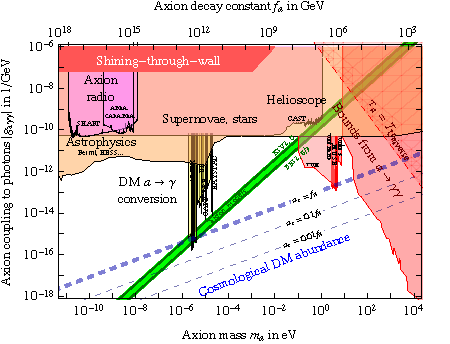
\includegraphics[width=0.68 \textwidth]{figs/assione} \end{center}
\caption[Axion phenomenology]{\em\label{fig:axion} {\bfseries Axion and axion-like particle phenomenology}. 
In the plane (axion mass, axion coupling to photons) we show
the range favoured by axion models (green band);
the initial axion vacuum expectation value $a_*$ that reproduces the observed DM abundance (blue dashed lines);
the exclusion bounds from non-observation of axion decays (upper-right red region)~\cite{axion:decay},
as well as absence of signals in shining-trough-wall experiments (upper-left red region)~\cite{ALPS,OSQAR,CROWS},
searches for axion emissions from the Sun (upper red region)~\cite{CAST,IAXO}, 
stars, dwarfs and supernov\ae{} (upper orange region)~\cite{axioncooling},
and axion DM conversion into photons (yellow regions)~\cite{ADMX,HAYSTAC,QUAX,CAPP}.
The bounds are discussed in more details in the main text; additional and much more refined bounds are collected at
\href{https://github.com/cajohare/AxionLimits}{github.com/cajohare/AxionLimits} (2024).}
\end{figure}

% should add https://arxiv.org/pdf/2503.11753 and 

\subsection{Searching for axion Dark Matter}
\label{AxionExp}
\index{Axion!detection}
\index{Axion-like particles}

In this section we discuss the phenomenology of the searches for axion and axion-like particles (ALPs). 
As already mentioned before (see the general discussion in section \ref{ultralight}), the basic difference between the two is that for axions the mass and the couplings to the SM particles are related via the symmetry breaking scale $f_a$, while ALPs are the generalization of this concept, where the link between the mass and couplings is relaxed. 
For simplicity, we will use in the rest of this section  the term axion in a broad sense, which includes ALPs.

\medskip

Axions must couple to gluons, and are expected to also couple to the other SM fields. 
The axion Lagrangian of eq.\eq{axioncouplings} results at low energies, $\mu\lesssim $ few GeV, in the following couplings to gluons, photons, quarks and leptons, 
\beq\label{eq:effective:axion:Lag}
\bbox{\Lag_{\rm axion}^{\rm eff} =\Lag_{\rm QCD}+
\frac{a}{f_a}\frac{\alpha_{\rm s}}{8\pi}G_{\mu\nu}^a\tilde G^{a,\mu\nu}+c_\gamma \frac{a}{f_a} \frac{\alpha}{2\pi} F_{\mu\nu}\tilde F^{\mu\nu} +
\frac{\partial_\mu a}{2f_a}\sum_{ij}\bar \Psi_i \gamma^\mu \big[C_{ij}^V+C_{ij}^A\gamma_5\big]\Psi_j}~,
\eeq
where the sum is over three types of neutral currents, 
either over up-quarks, $\Psi_i=u,c$, down-quarks, $\Psi_i=d,s,b$, or leptons $\Psi_i=e, \mu, \tau$.
Unlike in eq.~\eqref{eq:axioncouplings} they are written in Dirac notation, and
we kept the flavor-violating couplings, 
which can either result from integrating out the $W$ or are already present in the high-energy physics.  
Note that for $i=j$ the derivative couplings to vector currents do not contribute due to vector current conservation, so effectively one can set $C_{ii}^V=0$.


\paragraph{Searches relying on axion couplings to photons.} 
The axion almost inevitably couples to photons. If nothing else, the axion-gluon interaction induces at low energies the axion couplings to charged pions, and this in turn results in axion couplings to photons through loop corrections, see eq.~\eqref{eq:cgamma:axion} below. 
The axion coupling to photons, eq.\eq{gagammagamma1},  is the most important for axion phenomenology and is usually written as
\beq 
\Lag_{a\gamma\gamma} = 
-\frac{g_{a\gamma\gamma}}{4}  a F_{\mu\nu} \tilde F_{\mu\nu} = g_{a\gamma\gamma} a \mb{E}\cdot\mb{B},\qquad
\qquad
g_{a\gamma\gamma} = \frac{\alpha c_\gamma}{2\pi f_a},
\label{eq:gagammagamma}
\eeq
where $\tilde F_{\mu\nu} \equiv \frac{1}{2}\epsilon_{\mu\nu\alpha\beta}F_{\alpha \beta}$.
The constant $ g_{a\gamma\gamma}$ has dimension mass$^{-1}$ and
$c_\gamma$ is a model-dependent order one number.  Its explicit value, in the basis where the $aG\tilde G$ coupling
is rotated away (as discussed below eq.\eq{Qshift}) is 
\beq 
\label{eq:cgamma:axion}
c_\gamma = c_{\gamma,{\rm uv}}-\frac{2}{3}\frac{4+m_u/m_d+m_u/m_s}{1+m_u/m_d+m_u/m_s}
\approx c_{\gamma,{\rm uv}}-1.93, 
\qquad \text{where} \qquad
 c_{\gamma,{\rm uv}}=\frac{\sum_f X_f q_f^2}{\sum_f X_f T_f^2}.
\eeq
The second term in $c_\gamma$ comes from the axion-gluon interaction, while $c_{\gamma,{\rm uv}}$ is due to the triangle anomaly (with $a$ and two $\gamma$ as external legs) mediated by a loop of heavy  fermions charged 
under both the global PQ symmetry and under the $\U(1)_{\rm em}$ gauge symmetry. 
The sums in $c_{\gamma,{\rm uv}}$ are over Weyl fermions with PQ charges $X_f$ and electric charges $q_f$.
The denominator appears because, by convention, $f_a$ is normalized relative to the QCD triangle anomaly (with $a$ and two $g$ as external legs). 
The QCD anomaly receives contributions only from colored fermions, where $\Tr T^a T^b = T^2\delta^{ab}$, with $T^a$ the SU(3) generators in the appropriate representation. 
For SU(3) triplets one has $T^2=1/2$, and thus
DFSZ models, in which only SM fermions contribute to the anomaly, predict
\beq  c_{\gamma,{\rm uv}}
= \frac{ N_c(q_d^2 + q_u^2) + q_e^2}{1/2+1/2}=\frac83 \eeq
where $N_c=3$ is the number of colors in the SM, and we assumed that heavy fermions $f$ have common PQ charges $X_f$. 
For DFSZ models thus the two terms combine to $c_\gamma\simeq 0.73$, confirming the expectation that typically, $c_\gamma\sim 1$. 
KSVZ models too predict $E/N=8/3$ whenever the extra heavy fermions fill multiplets under the SU(5) unification gauge group
with common PQ charge.

Treating the background axion density as a classical field $a(x)$, see section~\ref{LightBosonDM}, 
the inhomogeneous Maxwell equations get modified to
\beq \mb{\nabla}\cdot\mb{E}= \rho  - g_{a\gamma\gamma}\mb{B}\cdot\mb{\nabla}a,\qquad
\mb{\nabla}\times\mb{B}=\mb{J} + \dot{\mb{E}} + g_{a\gamma\gamma} (\mb{B}\dot a -\mb{E}\times\mb{\nabla} a).\eeq
These re-acquire the Maxwell form if one defined the modified electric and magnetic fields,  
$\mb{E}'=\mb{E} +  g_{a\gamma\gamma}a \mb{B}$, 
$\mb{B}' = \mb{B} -  g_{a\gamma\gamma}a \mb{B}$. 
This shows that a varying axion field is able, in the presence of a background magnetic field, to produce electromagnetic effects such as electromagnetic waves, which can then be searched for.

\medskip

Axions remain unobserved, implying that the scale $f_a$ suppressing the axion interactions with the SM fields, including $g_{a\gamma\gamma}$, see eq.s~\eqref{eq:effective:axion:Lag} and \eqref{eq:gagammagamma}, must be very large.
Fig.\fig{axion} summarizes in the ($m_a,g_{a\gamma\gamma}$) plane the rich axion phenomenology and the current bounds from many axion searches, while table \ref{tab:AxionPhotonexp} lists some of the main laboratory experiments leading  to these bounds.
Below, we provide a concise overview of the key aspects highlighted in
fig.\fig{axion}.
\begin{itemize}
\item[\scalebox{0.6}{$\blacksquare$}]
The green band indicates the parameter space region predicted by the axion models according to eq.s\eq{maxion} and\eq{gagammagamma}. However,
its width is somewhat arbitrary, and would change with more complicated field content,  see, e.g., the discussion in \cite{DiLuzio:2016sbl}.

\item[\scalebox{0.6}{$\blacksquare$}] The blue dashed contour-lines show the initial axion vacuum expectation value $a_*$ that is required in order  to reproduce the observed cosmological DM abundance
via the misalignment mechanism, discussed in section~\ref{ultralight}, see also eq.~\eqref{eq:Omegaaxion}
(to convert $f_a$ into $g_{a\gamma\gamma}$ we assumed $c_\gamma = 1$).
The values $a_* \sim f_a$ (thick dashed line) are likely to be the more plausible ones.
\end{itemize}



\noindent The experimental constraints shown in fig.\fig{axion} are as follows.
\begin{itemize}
\item[$-$] The $a\gamma\gamma$ interaction leads to the {\bf axion decay} $a\to\gamma\gamma$. The corresponding lifetime 
\beq 
\label{eq:axion:lieftime}
\tau(a\to\gamma\gamma)=\frac{64\pi}{g_{a\gamma\gamma}^2 m_a^3}\approx T_{\rm U}\left(\frac{20\eV}{m_a}\right)^5,
 \eeq
must be
longer than the age of the universe, $T_{\rm U}$. The most stringent bounds  on the axion decay time are in fact much stronger, in the range
$\tau > 10^{21-26}\,{\rm s}$, depending on the value of the axion mass $m_a$, and follow  
 from the searches for an excess  of such photons, and from bounds on the re-ionization of the Universe. These give the upper-right red excluded region in fig.\fig{axion} \cite{axion:decay}.

If the axion mass is around 1 eV,  $a\to\gamma\gamma$ decays produce a flux of infrared or visible photons, which can be directly constrained by telescope observations such as {\sc Vimos}, {\sc Muse}, {\sc Winered}, {\sc Jwst}~\cite{axion:decay}.

\item[$-$] Laboratory experiments searching for {\bf light shining through wall} (photon--to--axion--to--photon conversion in a magnetic field)  \cite{ALPS,OSQAR,CROWS}
presently set the weak bound in the top-left part of fig.\fig{axion}.
These searches will be improved by the upcoming experiment ALPS-II.
\index{Light shining through wall}\index{Axion!light shining through wall}

\item[$-$] The strong horizontal bound in the upper part of fig.\fig{axion}, $g_{a\gamma\gamma}\circa{<}0.7~10^{-10}/\GeV$, comes from the absence of excessive {\bf cooling of stars} (including the Sun) and supernov\ae, due to axion production.
The axion cooling modifies the seismic properties of the star, its neutrino emission and in general its evolution. 
The former two effects, applied to the Sun, imply the bound $g_{a\gamma\gamma}\circa{<}{\rm few}~10^{-10}/\GeV$. 
The more stringent constraint quoted above comes from analyzing the number ratio $R$ of stars in the horizontal branch (HB) over the red giant branch (RGB) in old galactic globular clusters. 
This ratio would be modified (reduced) by the axion production from photon conversions occurring in the stellar cores~\cite{axioncooling}.

Notice also that the constraints from stellar and supernova cooling mentioned in section \ref{sec:mediators-sub-eV} apply~\cite{stellar:cooling,SN:constraints}, typically to masses larger than those considered in fig.\fig{axion}. 
Other stellar and supernova physics bounds on relatively heavy ALPs are considered in \cite{otherSNboundsonALPs}.

\item[$-$]
The more stringent bound $g_{a\gamma\gamma}\circa{<}{\rm few}~10^{-12}/\GeV$ at $m_a \lesssim 10^{-6}$ eV comes from the non-detection of irregularities in the spectra of a number of diverse astrophysical sources (quasars, blazars, clusters or individual galaxies)~\cite{axionconversion}. The photons emitted by these sources could {\bf convert into axions} while crossing intergalactic magnetic fields.
At a fundamental level this is the $\gamma\gamma \to a$ process, where the second $\gamma$ is the magnetic field. 
The conversion would dim the apparent intensity of the source, but this does not lead to testable effects given the uncertain randomness of the magnetic field and of the sources. 
It would also induce oscillatory features in the spectra of the sources, which are otherwise expected to be smooth, and this constitute a statistically testable signal.
\index{Axion!conversion of high-energy photons}  
Bounds at different axion masses are derived from different $\gamma$- and $X$-ray experiments (e.g.~{\sc Hess}, {\sc Fermi}, {\sc Magic}, {\sc Chandra})~\cite{axionconversion}. 

Still in the vein of conversion, other bounds can be derived from the non-observation of excess $X$-rays or radio-waves from relatively $X$-dim or radio-quiet sources~\cite{axionconversion2}. If these sources emit axions, these could {\bf convert into photons} in the magnetic fields along the way.
At particle level, the process is now  $a\gamma \to \gamma$, where the $\gamma$ in the initial state is the magnetic field. 
This is particularly efficient in the intense magnetic fields surrounding neutron stars. 
The non-observation of excess radio emission from pulsars (rotating neutron stars), or excess $X$-ray emission from Betelgeuse or some white dwarfs, or even of an excess in the $\gamma$-ray background from past supernov\ae\ allows to impose $g_{a\gamma\gamma}\circa{<}{\rm few}~10^{-11-12}/\GeV$ in various mass ranges, comparable to the stellar cooling bounds~\cite{axionconversion2}.

\index{Axion!conversion to high-energy photons}
A hint of a positive signal due to axion-photon conversion in some isolated neutron stars (known as the {\em Magnificent Seven}) is however claimed by \arxivref{1910.04164}{Bushmann et al.~(2019)}\ in~\cite{axionconversion2}.


\index{Axion!helioscope}\index{Sun!axion}
\item[$-$] While the Sun is not the hottest star, its proximity allows for
{\bf helioscope} experiments \cite{Sikivie:1983ip}, which
use intense magnetic fields to search for conversions of axions, emitted by the Sun, into photons (again $a\gamma\to\gamma$, where now the $\gamma$ in the initial state is the strong magnetic field in the experiment).
Helioscopes (such as CAST~\cite{CAST})  set bounds similar to the stellar cooling ones for $m_a\circa{<}0.02\eV$.
Future improvements are planned: the International Axion Observatory (IAXO) should improve the CAST reach on $f_a$ by more than an order of magnitude, surpassing the stellar cooling bounds \cite{IAXO}.

Observations of the Sun can also be used to impose constraints on axions in a different mass range, $m_a \approx 10$ keV. 
For these masses, a significant fraction of axions thermally produced in the solar core would possess a speed below the escape velocity and would remain gravitationally bound to the Sun, thereby accumulating in a {\bf solar axion basin}, eventually decaying into $X$-rays outside the Sun~\cite{axionsolarbasin}. 
$X$-ray observations imply the constraint $g_{a\gamma\gamma}\circa{<}{\rm few}~10^{-13}/\GeV$ (not shown in fig.\fig{axion}).
\index{Axion!solar basin}

\index{Axion!haloscope}
\item[$-$] {\bf Haloscope} experiments \cite{Sikivie:1983ip} use the $a\gamma\gamma$ coupling to search for resonant
conversion of galactic axion DM into a microwave photon with energy
$E_\gamma=m_a$ using a microwave cavity of volume $V$,
permeated by a strong magnetic field $B_0$.
The power generated within the cavity by axion to photon conversion is given by
\beq W = g_{a\gamma\gamma}^2 V B^2_0 \frac{\rho_\odot}{m_a} C \min (Q_{\rm cavity}, Q_{\rm axion}),
\eeq
where $C$ is a geometric factor (e.g.,\ $C=0.69$ for the TM$_{010}$ mode of
a cylindrical cavity permeated by a longitudinal $B_0$),
$Q_{\rm cavity}$ is the quality factor of the cavity and the inverse of
$Q_{\rm axion}$ measures the spread in the axion energy $E_a \simeq m_a c^2 + \frac{1}{2}m_a v^2$, so that
$Q_{\rm axion} \approx  (c/v)^2\approx 10^6$.
Streams of axions with common velocity would all have the same energy, which would then enhance the signal-to-noise ratio.

By varying the resonant frequency of the cavity one can probe different axion masses
(yellow dips in fig.\fig{axion}). These searches already reach the sensitivity to the parameter space predicted by the most popular axion models,
but only in narrow ranges of axion masses, because relatively long running times are needed at each frequency in order to accumulate sufficient signal.
Recent and current haloscopes include {\sc RBF, UF, ADMX, Haystac, Quax-$a\gamma$, Capp} \cite{RBF,ADMX,HAYSTAC,QUAX,CAPP}, as well as many others (see table \ref{tab:AxionPhotonexp}).


\end{itemize}
There are also a number of other experimental approaches, 
some of which target axion masses that are not  in the ranges considered to be the most plausible
(see \cite{axionreviews} for further details):
\begin{itemize}

\item[$-$]
{\bf Dish antennae and dielectric haloscopes}. 
If an external magnetic field is aligned along a conducting surface, such as a mirror, or a surface of a block of dielectric material, the oscillating DM axion field excites the electrons inside the material, 
leading to the emission of electromagnetic radiation from the  surface of the material.  
Future searches for the electromagnetic radiation emitted by large surface magnetised dish antennae and dielectric haloscopes, such as {\sc Madmax}, consisting of a large array of dielectric slabs, are expected to reach considerable sensitivity~\cite{MADMAX}.  


\item[$-$]
{\bf Axion DM radios}. The oscillating DM axion field in a constant external magnetic field induces a small oscillating $\mb{B}$ field. 
This can then be detected using pick-up coils inside a larger magnet. 
Table top size experiments based on this idea (e.g.,~{\sc Abracadabra}) placed limits 
comparable to those from the CAST helioscope, down to axions masses $m_a\sim 10^{-8-10} \eV$.
This technique could reach sensitivities around the QCD axion band in fig.~\ref{fig:axion} for axions lighter than about $1\,\mu$eV,
if magnets with $B \sim \hbox{few T}$ and of cubic meter volumes can be used in the future~\cite{axion:DM:radios,ABRACADABRA,SHAFT,BASE,DMRadio}. \\
A similar technique, using the whole Earth as the test volume, has been used to impose constraints on very light axions or dark photons ($m_a \sim 10^{-17}$ eV), using data from the {\sc SuperMAG} Collaboration \cite{SuperMAG}, and on slightly heavier axions ($m_a \sim 10^{-14}$ eV) in \cite{Taruya:2025zql}.

\item[$-$]
{\bf Polarization experiments}. Photon-axion conversions in the presence of an external magnetic field $\mb{B}$ would reduce the 
polarization component of a laser beam parallel to $\mb{B}$ (dichroism) and delay its phase (birefringence).
This effect has been searched for, e.g.,~by {\sc Pvlas}~\cite{PVLAS}, obtaining relatively weak bounds, $|g_{a\gamma\gamma}|\circa{<}10^{-7}/\GeV$.

\item[$-$] {\bf Gravitational wave experiments} allow to probe axions and other ultra-light DM candidates coupled to photons~\cite{GWexpDM}.
\end{itemize}




\begin{table}[!p]
  \begin{center}
    \setlength\tabcolsep{1pt} \renewcommand{\arraystretch}{0.95}
     \resizebox{\columnwidth}{!}{
      \begin{tabular}{ccccccclrcc}
        \hline
        \hline
        {\bf Experiment}  & {\bf Location}
                          & {\bf Operation}       & {\bf Technology}
                          & \multicolumn{4}{c}{\bf Mass Range}        & {\bf Coupling~}                   & ~~{\bf Home}~~
                          & {\bf Ref.} \\
          & &  &  & \multicolumn{4}{c}{ } & {\bf sensitivity}   &  &  \\       
          & &  &  & \multicolumn{4}{c}{ } & (GeV$^{-1}$)~  &  &  \\       
                  \hline

        \rule{0pt}{1ex}
        {\sc SuperMAG} & Worldwide & 1970 $\to$ ~~~~ & Magnetic Field HS & 2 & $\to$ & 70 & aeV & $6.5\ 10^{-11}$ &\href{https://supermag.jhuapl.edu/}{web} & \cite{SuperMAG}
        \\

        %RBF - 2
        \rule{0pt}{1ex}
        {\sc RBF} & BNL, USA  & 1987 & $\mu$-wave Cavity HS & 4.5 & $\to$ & 5.0 &$\mu$eV & $10^{-11}$ & $-$ &\cite{RBF}
        \\

        %UF - 3
        \rule{0pt}{1ex}
        {\sc UF} & UoFlorida, USA & 1989 & $\mu$-wave Cavity HS & 5.4 &$\to$ & 5.9 & $\mu$eV & $3.7\ 10^{-14}$ & $-$ & \cite{UF}
        \\

        %ADMX - 4
        \rule{0pt}{1ex} 
        \multirow{2}{*}{{\sc ADMX}~~$\Big\{$}
        & LLNL, USA
        & 1995 $\to$ 2010  & \multirow{2}{*}{$\mu$-wave Cavity HS} & 1.9 &$\to$ &3.69 &$\mu$eV & $ 1\ 10^{-15}$ & \multirow{2}{*}{\href{https://depts.washington.edu/admx/}{web}} & \multirow{2}{*}{\cite{ADMX}}
        \\
        \rule{0pt}{1ex}
        & CENPA, USA & 2017 $\to$ ~~~~& & 2.66 &$\to$ &4.2 &$\mu$eV & $ 3.5\ 10^{-16}$& & 
        \\

        %CAST - 5
        \rule{0pt}{1ex}
        \multirow{2}{*}{CAST} & \multirow{2}{*}{CERN~~$\Big\{$} & 2004 & \multirow{2}{*}{Helioscope} & &$\lesssim$ & 20 & meV & $8.8\ 10^{-11}$ &\multirow{2}{*}{\href{http://cast.web.cern.ch/CAST/}{web}} & \multirow{2}{*}{\cite{CAST}}
        \\
    & & 2013 $\to$ 2015 & & &$\lesssim$ & 20 & meV & $6.6\ 10^{-11}$ & & 
    \\

        %ALPS - 6
        \rule{0pt}{1ex}
        \multirow{2}{*}{\sc ALPS} & \multirow{2}{*}{DESY, Germany~~$\Big\{$} & 2007 $\to$ 2010 & \multirow{2}{*}{LSW} & &$\lesssim$ & $1$ & meV & $7\ 10^{-8}$ &\multirow{2}{*}{\href{https://alps.desy.de/}{web}} & \multirow{2}{*}{\cite{ALPS}}
        \\
        & & 2023? & & &$\lesssim$ & $1$ & meV & $2\ 10^{-11}$ & & 
        \\

        %CROWS - 7
        \rule{0pt}{1ex}
        {\sc Crows} & CERN & 2013 & Microwave LSW & &$\lesssim$ & 7.2 &$\mu$eV & $4.5\ 10^{-8}$ & $-$ &\cite{CROWS} 
        \\

        %OSQAR - 8
        \rule{0pt}{1ex}
        {\sc Osqar} & CERN & 2014 & LSW & &$\lesssim$ & 0.2 &meV & $3.5\ 10^{-8}$ &\href{https://home.cern/science/experiments/osqar}{web} & \cite{OSQAR}
        \\

        %PVLAS - 9
        \rule{0pt}{1ex}
        {\sc Pvlas} & Padova, Italy & 2015 & Optical Birefringence & &$\lesssim$ & 0.01 &eV & $1\ 10^{-7}$ &\href{https://en.wikipedia.org/wiki/PVLAS}{wiki} & \cite{PVLAS}
        \\

        %ADMX Sidecar - 10
        \rule{0pt}{1ex} 
        {\sc ADMX Sidecar} & CENPA, USA & 2016 $\to$ ~~~~ & $\mu$-wave Cavity HS & 17.38 &$\to$ &29.79 &$\mu$eV & $2.6\ 10^{-13} $ & \href{https://depts.washington.edu/admx/}{web} & \cite{ADMX} 
        \\

        %HAYSTAC - 11
        \rule{0pt}{1ex}
        {\sc Haystac} & Yale, USA & 2016 $\to$ 2021 & $\mu$-wave Cavity HS & 16.96 &$\to$ & 24.0 &$\mu$eV & $9.07\ 10^{-15}$ &\href{https://haystac.yale.edu/}{web} &\cite{HAYSTAC}
        \\

        %ORGAN - 12
        \rule{0pt}{1ex}
        {\sc Organ} & UWA, Australia & 2017 $\to$ 2022& $\mu$-wave Cavity HS &63.2 &$\to$ &110 &$\mu$eV & $2.02\ 10^{-12}$ & $-$ &\cite{ORGAN}
        \\

        % ABRACADABRA - 13
        \rule{0pt}{1ex}
        {\sc Abracadabra}  & MIT, USA & 2018  & Lumped Element HS & 0.31 &$\to$ &8.3 &neV  & $3.2 \  10^{-11} $  & \href{https://abracadabra.mit.edu/abracadabra}{web} & \cite{ABRACADABRA}
        \\

        %ADMX SLIC - 14
        \rule{0pt}{1ex} 
        {\sc ADMX SLIC} & UoFlorida, USA & 2018 & Lumped Element HS & 0.175 &$\to$ & 0.180 &$\mu$eV & $10^{-12}$ & \href{https://depts.washington.edu/admx/}{web} & \cite{ADMX}
        \\
        
        %QUAX - 15
        \rule{0pt}{1ex}
        {\sc QUAX-$a\gamma$} & LNL, Italy & 2018 $\to$ 2021 & $\mu$-wave Cavity HS &37.5 & $\to$ &42.8 &$\mu$eV & $7.31\ 10^{-14}$ & \href{https://www.pd.infn.it/eng/quax/}{web} & \cite{QUAX}
        \\

        %RADES -16
        \rule{0pt}{1ex}
        {\sc RADES} & CERN & 2018 & RF Cavity HS & & $\simeq$ & 34.67 & $\mu$eV &$4\ 10^{-13}$ & \href{https://www.mpp.mpg.de/en/research/rades-detector}{web} & \cite{RADES}
        \\

        %CAPP - 17
        \rule{0pt}{1ex} 
        {\sc CAPP} & {CAPP, S.~Korea} & 2019 $\to$ ~~~~ & $\mu$-wave Cavity HS & 4.5 &$\to$ &19.9 &$\mu$eV & $ \sim 10^{-15} $ & \href{https://capp.ibs.re.kr/html/capp_en/}{web}  & \cite{CAPP}
        \\

        %CAST-CAPP - 18
        \rule{0pt}{1ex} 
        {\sc CAST-CAPP} & CERN & 2019 $\to$ 2021 & $\mu$-wave Cavity HS & 19.74 &$\to$ &22.47 &$\mu$eV & $8\ 10^{-14}$ & \href{http://cast.web.cern.ch/CAST/index.php}{web}  & \cite{CAST-CAPP}
        \\

        %SHAFT -19
        \rule{0pt}{1ex}
        {\sc SHAFT} & Boston Univ. & 2019 & Lumped Element HS & 12 &$\to$ &12$\ 10^3$ & peV & $4\ 10^{-11}$ & $-$ &\cite{SHAFT}
        \\

        %UPLOAD - 20
        \rule{0pt}{1ex}
        \multirow{2}{*}{\sc UPLOAD} & \multirow{2}{*}{UWA, Australia~~$\Big\{$} & $2019^{\dagger}$ &\multirow{2}{*}{$\mu$-wave Cavity HS} & 7.44 &$\to$ &19.38 &neV & $3\ 10^{-13}$ & \multirow{2}{*}{$-$} &\multirow{2}{*}{\cite{UPLOAD}}
        \\
        & & $2023^{\dagger}$ & & 1.12 &$\to$ & 1.20 &$\mu$eV & $3\ 10^{-6}$ & & 
        \\

        %BASE - 21
        \rule{0pt}{1ex} 
        {\sc BASE} & CERN & $2020^{\dagger}$ & Penning Trap HS & &$\simeq$ &2.79 &neV & $10^{-11}$ & \href{https://base.web.cern.ch/content/base-experiment}{web}  &\cite{BASE}
        \\

        %DANCE - 23
        \rule{0pt}{1ex}
        \multirow{2}{*}{\sc DANCE} & \multirow{2}{*}{UoTokyo, Japan ~~$\Big\{$ } & 2021 & \multirow{2}{*}{Optical Cavity HS} & $10^{-14}$ &$\to$ &$10^{-13}$ &eV &$8\ 10^{-4}$  & \multirow{2}{*}{\href{https://granite.phys.s.u-tokyo.ac.jp/oshima/presentation/KashiwaDM_Oshima_ver3.pdf}{slides}}  & \multirow{2}{*}{\cite{DANCE}}
        \\
        & & Proposed & & &$\lesssim$& $10^{-10}$ &eV & $3\ 10^{-16}$ 
        & &
        \\ 

        %GrAHal - 24
        \rule{0pt}{1ex}
        \multirow{2}{*}{\sc GrAHal} & \multirow{2}{*}{Grenoble, France~~$\Big\{$ } & 2021 & \multirow{2}{*}{$\mu$-wave Cavity HS} & &$\simeq$ &26.37 &$\mu$eV & $2.2\ 10^{-13}$ & \multirow{2}{*}{\href{https://grahal.neel.cnrs.fr/}{web}} & \multirow{2}{*}{\cite{GrAHal}}
        \\
        & & 2023? & & 1.25 &$\to$ &125 &$\mu$eV & $1.1\ 10^{-14}$ & &
        \\

        %LAMPOST - 25
        \rule{0pt}{1ex}
        {\sc Lampost} & MIT, US & 2021 & Optical Dielectric HS & 0.1 &$\to$ &10 &eV & $\sim 10^{-12}$ & $-$ &\cite{LAMPOST}
        \\

        %TASEH - 26
        \rule{0pt}{1ex}
        {\sc Taseh} & NCU, Taiwan & 2021 & $\mu$-wave Cavity HS &  &$\simeq$ & 19 &$\mu$eV & $8.2\ 10^{-14}$ &\href{http://taseh.phy.ncu.edu.tw/}{web} & \cite{TASEH}
        \\

        %SAPPHIRE - 27
        \rule{0pt}{1ex}
        {\sc Sapphires} & Kyoto Univ., Japan &  $2022^{\dagger}$ & Laser Collider &0.005 &$\to$ &0.5 & eV & $1.14\ 10^{-5}$ &\href{https://www.spphrs.hiroshima-u.ac.jp/index.html}{web} &\cite{SAPPHIRES}
        \\

        %WISPLC - 28
        \rule{0pt}{1ex}
        {\sc WISPLC} & UHH, Germany & 2023? & Lumped Element HS & $10^{-11}$ &$\to$ & $10^{-6}$ & eV & $10^{-15}$ &\href{https://www.physik.uni-hamburg.de/en/iexp/gruppe-horns/forschung.html}{web} & \cite{WISPLC}
        \\

        %BabyIAXO - 29
        \rule{0pt}{1ex}
        {\sc Baby-IAXO} & DESY, Germany & 2024? & Helioscope & &$\lesssim$ & 0.25 & eV & $1.5\  10^{-11}$ &\href{https://iaxo.desy.de/}{web} & \cite{IAXO}
        \\

%        %ADD - 29b
%        [no paper yet, only a poster at a conference in Tokyo in sept 2025]
%        \rule{0pt}{1ex}
%        {\sc Add} & CERN, Switzerland & 2028? & RF Cavity HS & $4 \, 10^{-11}$ &$\to$ & $4 \, 10^{-9}$ & eV & $\sim 10^{-15}$ &\href{}{web} & \cite{}
%        \\

        %IAXO - 30
        \rule{0pt}{1ex}
        {\sc IAXO} & DESY, Germany & 2030? & Helioscope & &$\lesssim$ & 1 & eV & $10^{-12}$ & \href{https://iaxo.desy.de/}{web} &\cite{IAXO}
        \\

        %MADMAX - 31
        \rule{0pt}{1ex}
        {\sc Madmax} & DESY, Germany & 2030? & Dielectric HS & 40 &$\to$ & 400 &$\mu$eV & $10^{-14}$ & \href{https://madmax.mpp.mpg.de/index.html}{web} & \cite{MADMAX}
        \\

        %BREAD - 32
        \rule{0pt}{1ex} 
        {\sc Bread} & Fermilab, USA & Pilot & Dish Antenna HS & $10^{-4}$ &$\to$ &1 &eV & $\sim10^{-13}$ & $-$ & \cite{BREAD}
        \\       

        %CADEx - 33
        \rule{0pt}{1ex} 
        {\sc CADEx} & LSC, Spain & Prep. & $\mu$-wave Cavity HS & 330 &$\to$ &460 &$\mu$eV & $ 3\ 10^{-13} $ & \href{https://lsc-canfranc.es/wp-content/uploads/2022/01/CADEx_presentation_V0.pdf}{slides} &\cite{CADEx}
        \\

        %WISPFI - 34
        \rule{0pt}{1ex}
        {\sc WISPfi} & UHH, Germany & Constr. & Fiber Interferometer & 50 &$\to$ & 100 & meV & $ 10^{-11}$ & \href{https://www.physik.uni-hamburg.de/en/iexp/gruppe-horns/forschung.html}{web} & \cite{WISPFI}
        \\

        %DMRadio - 39
        \rule{0pt}{1ex}
        {\sc DMRadio} & SLAC, USA & Constr. & Lumped Element HS &$0.02$ &$\to$& $830$ &neV & $10^{-17}$  & \href{https://irwinlab.stanford.edu/dark-matter-radio-dm-radio}{web}  & \cite{DMRadio}
        \\

        %aLIGO - 35
        \rule{0pt}{1ex} 
        {\sc aLIGO} & LIGO, USA & Proposed & Optical Cavity HS & $10^{-16}$ &$\to$ &$10^{-9}$ &eV & $8.3\  10^{-13} $ & \href{https://advancedligo.mit.edu/}{web} & \cite{aLIGO}
        \\

        %ALPHA - 36
        \rule{0pt}{1ex} 
        {\sc ALPHA} & Stockholm Univ., Sweden & Proposed & Plasma HS & 35 &$\to$ &400 &$\mu$eV & $\sim 10^{-14}$ & \href{https://axiondm.fysik.su.se/alpha/}{web}  & \cite{ALPHA}
        \\

        %BRASS - 37
        \rule{0pt}{1ex} 
        {\sc BRASS} & Hamburg, Germany & Proposed & Broadband HS & 10 &$\to$ &$10^{4}$ &$\mu$eV & $-$~~ & \href{https://www.physik.uni-hamburg.de/iexp/gruppe-horns/forschung/brass.html}{web} & $-$
        %website only
        \\

        %DALI - 38
        \rule{0pt}{1ex}
        {\sc Dali} & Teide Observatory, Spain & Proposed & Dielectric HS & 25 &$\to$ &250 &$\mu$eV & $3.75 \ 10^{-15}$ & \href{https://www.iac.es/en/projects/dalipop-pioneering-tunable-broad-band-search-axion-dark-matter-above-25-mev}{web}  &\cite{DALI} 
        \\

        %KLASH/FLASH - 40
        \rule{0pt}{1ex}
        {\sc Flash} & LNF, Italy & Proposed & $\mu$-wave Cavity HS & 0.2 &$\to$ & 1 &$\mu$eV & $5.3\ 10^{-15}$ & \href{https://coldlab.lnf.infn.it/experiments/klash/}{web}  & \cite{KFLASH}
        \\

        %SRF - 42
        \rule{0pt}{1ex}
        {\sc SRF/Dark-SRF} & Fermilab, USA? & Proposed & Supercond. RF HS & $10^{-22}$ &$\to$ & $10^{-7}$ & eV & $10^{-18}$ & \href{https://news.fnal.gov/tag/srf/}{web} & \cite{SRF}
        \\

        %TOORAD - 43
        \rule{0pt}{1ex}
        {\sc Toorad} & Padova, Italy & Proposed & Topol. Magn. Ins. HS & 1 &$\to$ & 10 & meV &$ 4\ 10^{-12\, \ddagger}$ & \href{https://researchoutreach.org/articles/searching-axions-revealing-dark-matter-particle/}{article} & \cite{TOORAD}
        \\

        \hline\hline
      \end{tabular}}
  \end{center}
  \caption[Main axion-photon experiments]{\label{tab:AxionPhotonexp}\em Main {\bfseries axion search experiments}, sensitive to the {\bfseries axion-photon coupling $g_{a\gamma\gamma}$}, eq.~\eqref{eq:gagammagamma}. In the table, HS designates the {\em haloscopes}, while LSW designates the {\em light shining through a wall} experiments. The symbol $^\dagger$ indicates initial publication year in case the run period of experiment is not mentioned. The symbol $^\ddagger$ indicates that the sensitivity depends on the choice of the material. 
 We gratefully acknowledge the work of Aryaman Bhutani for the content of this table.
 }

\end{table}


\begin{table}[!th]

\begin{center}
    \setlength\tabcolsep{1pt} \renewcommand{\arraystretch}{0.95}
    \resizebox{\columnwidth}{!}{
      \begin{tabular}{ccccccclrcc}
        \hline\hline
        {\bf Experiment}  & {\bf Location}
                          & {\bf Operation}       & {\bf Technology}
                          & \multicolumn{4}{c}{\bf Mass Range}        & {\bf Coupling~~}                   & ~~{\bf Home}~~
                          & {\bf Ref.}
        \\
        \multicolumn{8}{c}{} & {\bf sensitivity } & & \\
        \multicolumn{8}{c}{} & (GeV$^{-1}$)~~ & & \\[1mm]
        \hline
        \\[-3mm]

        %nEDM - 1
        \rule{0pt}{1ex}
        {\sc nEDM} & Grenoble, France & 1998 $\to$ 2016 & neutron EDM & $10^{-24}$ &$\to$ &$10^{-17}$ &eV &$\sim4\ 10^{-5}$ & \href{https://www.ill.eu/news-press-events/press-corner/press-releases/ultra-cold-neutrons-aid-the-search-for-dark-matter-17112017}{article}& \cite{nEDM}
        \\

        % SNO - 2
        \rule{0pt}{1ex}
        {\sc SNO} & Sudbury, Canada~~& 1999 $\to$ 2006 & neutrino obs &  &$\lesssim$ & 5.5 &MeV & $1.88\ 10^{-15}$ & \href{https://sno.phy.queensu.ca/}{web} & \cite{SNOaxions}
        \\

        %K3He - 3
        \rule{0pt}{1ex}
        {\sc K-$^3$He Comagnetometer} & Princeton, USA & 2008 & Comagnetometer & 0.04 &$\to$ &40 &feV & $2.4\ 10^{-10}$ & $-$ & \cite{K3He}
        \\

        %PSI HgM - 4
        \rule{0pt}{1ex}
        {\sc PSI HgM} & PSI, Switzerland & 2017 & Spin Precession & $10^{-16}$ &$\to$ & $10^{-13}$ &eV & $3.5\ 10^{-6}$ & \href{https://www.psi.ch/en/ltp-ucn-physics/dark-matter-search}{web} & \cite{HGM}
        \\

        %CASPEr-ZULF - 5
        \rule{0pt}{1ex}
        {\sc CASPEr-ZULF} & Mainz, Germany & 2018 &  NMR/Comagnetometer & $10^{-22}$ &$\to$ & $7.8\ 10^{-14}$ &eV & $6\times10^{-5}$ & \href{https://budker.uni-mainz.de/?page_id=7}{web} & \cite{CASPER-ZULF}
        \\

        %JEDI - 6
        \rule{0pt}{1ex}
        {\sc Jedi} & J\"ulich, Germany & 2019 & Storage Ring & 0.495 &$\to$ & 0.502 &neV & $1.5\ 10^{-5}$ & \href{http://collaborations.fz-juelich.de/ikp/jedi/index.shtml}{web} & \cite{JEDI}
        \\

        %Hefei Xe129 - 7
        \rule{0pt}{1ex}
        {\sc Hefei Xe129} & Hefei, China  & 2021$^{\dagger}$ & Quantum Sensor & 8.3 &$\to$ & 744  &feV & $5.44\ 10^{-9}$ & $-$ & \cite{HEFEI}
        \\

        %NASDUCK Floquet - 8
        \rule{0pt}{1ex}
        {\sc NASDUCK Floquet} & Haifa, Israel & 2021 & Atomic Spin & $4\ 10^{-15}$ &$\to$ & $4\ 10^{-12}$ &eV & $1\ 10^{-7}$ & $-$ & \cite{NASDUCK}
        \\

        %NASDUCK SERF - 9
        \rule{0pt}{1ex}
        {\sc NASDUCK SERF} & Haifa, Israel & 2022 & Atomic Spin & $1.4\ 10^{-12}$ &$\to$ &$2\ 10^{-10}$ &eV & $5\ 10^{-6}$ & $-$ & \cite{NASDUCK-SERF}
        \\
        
        %ChangE - 10
        \rule{0pt}{1ex}
        {\sc ChangE} & Beijing, China & 2023 & Quantum Sensor & $4\ 10^{-17}$ &$\to$ & $4\ 10^{-12}$ &eV & $3\ 10^{-10}$ & $-$ & \cite{CHANGE}
        \\

        %CASPEr WIND - 11
        \rule{0pt}{1ex}
        {\sc CASPEr} & Mainz, Germany & Projection & NMR & $1\ 10^{-14}$ &$\to$ & $1\ 10^{-6}$ &eV & $\sim1\ 10^{-14}$ & \href{https://budker.uni-mainz.de/?page_id=7}{web} & \cite{CASPER}
        \\

        %He-3 HPD - 12
        \rule{0pt}{1ex}
        {\sc Superfluid He-3 HPD} & $-$  & Projection & NMR & 7 &$\to$ & 74 &neV & $\sim1\ 10^{-12}$ & $-$ & \cite{He-3_HPD}
        \\
        \hline\hline
      \end{tabular}
    }
  \end{center}
          \caption[Main axion-nucleon experiments]{\label{tab:AxionNexp}\em Main {\bfseries axion search experiments}, sensitive to the dimensionless {\bfseries axion-nucleon coupling $g_{aN}$}. In the table, HS designates a {\em haloscope}. The symbol $^\dagger$ indicates initial publication year in case the run period of experiment is not mentioned. We gratefully acknowledge the work of Aryaman Bhutani  for the content of this table.}
          


\begin{center}
    \setlength\tabcolsep{1pt} \renewcommand{\arraystretch}{0.95}
    \resizebox{\columnwidth}{!}{
      \begin{tabular}{ccccccclrcc}
        \hline\hline
        {\bf Experiment}  & {\bf Location}
                          & {\bf Operation}       & {\bf Technology}
                          & \multicolumn{4}{c}{\bf Mass Range}        & {\bf Coupling~}                   & ~~{\bf Home}~~
                          & {\bf Ref.}
        \\
        \multicolumn{8}{c}{ } & {\bf sensitivity} & & \\[1mm]
        \hline 
        \\[-3mm]

        %DARKSIDE-50 - 1
        \rule{0pt}{1ex}
        \multirow{2}{*}{\sc DarkSide-50} & \multirow{2}{*}{LNGS, Italy~~$\Big\{$} & \multirow{2}{*}{2013 $\to$ 2020} & \multirow{2}{*}{LAr}  & 30 &$\to$ &200 &eV &$5\ 10^{-13}$ & \multirow{2}{*}{\href{https://darkside.lngs.infn.it/}{web}}& \multirow{2}{*}{\cite{DarkSide-50}}
        \\
        & & & & 30 &$\to$ &20000 &eV &$1\ 10^{-12}$ & & 
        \\

        % LUX - 2
        \rule{0pt}{1ex}
        {\sc LUX} & Sanford, SD & 2013 & LXe & 1 &$\to$ & 16 &keV & $4.2\ 10^{-13}$ & \href{https://lux.brown.edu/}{web} & \cite{LUX}
        \\

        %EDELWEISSIII - 3
        \rule{0pt}{1ex}
        {\sc EDELWEISS-III} & LSM, France & 2014 $\to$ 2015 & Ge detector & 0.8 &$\to$ &500 &keV & $1\ 10^{-11}$ & \href{http://edelweiss.in2p3.fr/index.php}{web} & \cite{EDELWEISS-III}
        \\

        %PANDAX-II - 4
        \rule{0pt}{1ex}
        {\sc PandaX-II(solar)} & \multirow{2}{*}{~~Jinping, China~~$\Big\{$} & \multirow{2}{*}{2014 $\to$ 2019} & \multirow{2}{*}{LXe} & $10^{-2}$ &$\to$ & $10^{3}$ &eV & $4.35\ 10^{-12}$ & \multirow{2}{*}{\href{https://pandax.sjtu.edu.cn/}{web}} & \multirow{2}{*}{\cite{PandaX-I}}
        \\
        {\sc PandaX-II(galactic)} & & & & 1 &$\to$ &25  &keV & $4.3\ 10^{-14}$ & &
        \\

        %SUPERCDMS - 5
        \rule{0pt}{1ex}
        {\sc SuperCDMS} & Soudan, MN & 2014 $\to$ 2015 &  Ge detector & 0.04 &$\to$ & 500 &keV & $\sim10^{-12}$ & \href{https://supercdms.slac.stanford.edu/}{web} & \cite{CDMSlite}
        \\

        %GERDA - 6
        \rule{0pt}{1ex}
        {\sc Gerda} & LNGS, Italy & 2015 $\to$ 2018 &  Ge detector & 0.06 &$\to$ & 1 &MeV & $3\ 10^{-12}$ & \href{https://www.mpi-hd.mpg.de/gerda/}{web} & \cite{GERDA}
        \\

        %XENON1T - 7
        \rule{0pt}{1ex}
        {\sc XENON1T} & LNGS, Italy & 2016 $\to$ 2018 &LXe & 0.186 &$\to$ & 400 &keV & $5\ 10^{-15}$ & \href{https://xenonexperiment.org/}{web} & \cite{Xenon-1T}
        \\

        %QUAX-ae - 8
        \rule{0pt}{1ex}
        {\sc QUAX-$ae$} & LNL, Italy & 2018 $\to$ 2019 &~~YIG ferromagn.~HS~~& 4.4 &$\to$ &58 &$\mu$eV & $1.7\ 10^{-11}$ & \href{https://www.pd.infn.it/eng/quax/}{web} & \cite{QUAXae}
        \\

        %XENONnT - 9
        \rule{0pt}{1ex}
        {\sc XENONnT} & LNGS, Italy & 2021 & LXe & 1 &$\to$ &140 &keV & $\sim10^{-14}$ &\href{https://xenonexperiment.org/}{web} & \cite{XenonAnomaly}
        \\
        
        %Magnin Quantum Nondemolition - 10
        \rule{0pt}{1ex}
        {\sc Magnon QND} & UoTokyo, Japan & $2021^{\dagger}$ & magnon excitation & &$\simeq$ & 33.1 &$\mu$eV & $2.6\ 10^{-6}$ & $-$ & \cite{MagnonQND}
        \\

        %LUX ZEPLIN - 11
        \rule{0pt}{1ex}
        {\sc LZ} & Sanford, SD & 2022 $\to$ ~~~~ & LXe & 2 &$\to$ & 20 &keV & $1.5\ 10^{-13}$ & \href{https://lz.lbl.gov/}{web} & \cite{LZaxions}
        \\
        \hline\hline
      \end{tabular}}
  \end{center}
    \caption[Main axion-electron experiments]{\label{tab:AxionEexp}\em Main {\bfseries axion search experiments}, sensitive to the dimensionless {\bfseries axion-electron coupling $g_{ae}$}. In the table, HS designates a {\em haloscope}. The symbol $^\dagger$ indicates initial publication year in case the run period of experiment is not mentioned. We gratefully acknowledge the work of Aryaman Bhutani for the content of this table.}
\end{table}


\paragraph{Searches relying on couplings to gluons and/or SM fermions.} 
While most axion searches focus on couplings to photons, the axion couplings to gluons or SM fermions, see eq.~\eqref{eq:effective:axion:Lag}, can lead to additional signals.\footnote{The coupling to fermions can in turn also induce a two-photon coupling, via a fermionic triangle loop, see e.g.~\cite{SNboundsloop}.}
Tables \ref{tab:AxionNexp} and \ref{tab:AxionEexp} list the main experiments probing these other interactions. See also a similar, but more general, discussion in section \ref{sec:UDM:direct}.
\begin{itemize}
\item[\scalebox{0.6}{$\blacksquare$}] The axion couplings to gluons and quarks generate, at low energies, a coupling between the axion field and the nucleon spins. 
The most relevant operators are 
\beq
\label{eq:Laga:eff:gluons:quarks}
\Lag_a^{\rm eff} = g_{aN} (\partial_\mu a) \bar N \gamma^\mu \gamma_5 N-\frac{i}{2} g_{ad} \, a \bar N \sigma_{\mu\nu}\gamma_5 N F^{\mu\nu}.
\eeq
As discussed above, the local DM axion field oscillates with frequency determined by its energy $E_a \simeq m_a $, 
so that the first interaction sources an {\bf oscillating magnetic dipole} with coupling $g_{aN}\propto 1/f_a$, and the second an {\bf oscillating electric dipole}, with $g_{ad}\propto 1/m_N f_a$. 
For nonrelativistic nucleons, which is the case for nucleons bound inside a nucleus, the leading non-relativistic Lagrangian following from eq.~\eqref{eq:Laga:eff:gluons:quarks} is given by
\beq
\Lag_a^{\rm NR}=-\gamma_N \vec B_a^{\rm eff}\cdot \vec S_N,\qquad
\vec B_a^{\rm eff} =-\frac{2}{\gamma_N}[ g_{aN}\vec \nabla a+ g_{ad} a \vec E ] .
\eeq
Here, $\vec S_N$ is the spin of the nucleon, and $\vec E$ the electric field acting on the nucleon 
(for nucleons bound inside nucleus this differs from the applied external electric field due to shielding by the electronic cloud). 
The oscillating axion therefore plays the role of an effective magnetic field $B_a^{\rm eff}$,
where $\gamma_N$ is the gyromagnetic ratio of the nucleon. 
Such an oscillating axio-magnetic field can be detected via induced precession of nuclear spins, and can, in the future, be searched for via nuclear magnetic resonance techniques~\cite{axion:nEDM:oscill}. 
These experiments may in the long term reach the sensitivity to the nominal QCD axion band (the green band in figure~\ref{fig:axion}),
if $m_a\sim \mu$eV.

\item[\scalebox{0.6}{$\blacksquare$}] For flavor diagonal couplings to quarks, {\bf colliders} set bounds on axions (and more generic axion-like particles) that have relatively small decay constants, $f_a\sim \TeV$,
and therefore large masses, $m_a$, see sections~\ref{chapter:collider} and~\ref{sec:ALP:portal}.

\item[\scalebox{0.6}{$\blacksquare$}] {\bf Production in flavor violating decays}. 
Flavor violating axion couplings induce flavor-changing neutral current decays of quarks, 
such as $s\to d a$ and $b\to s a$, and of leptons, $\mu \to e a$ and $\tau \to e a, \mu a$ \cite{axion:flavor}. One can consider two limits: large and small flavor violating couplings. In the first case, i.e., if the flavor violating couplings are present in the full theory then generically  $C_{ij}^{A,V}\approx1$ and such decays give stringent bounds, typically 
above $f_a\gtrsim 10^9$ GeV. In this case the QCD axion is light, $m_a\ll$ eV (see eq.~\eqref{eq:maxion}), and has a cosmologically long lifetime (see eq.~\eqref{eq:axion:lieftime}). Decays such as $K\to \pi a$ and $B\to Ka$ therefore appear in the experiments as decays with missing energy, 
since the axions escape the detector before decaying. 
The resulting bounds are comparable or even more stringent than the astrophysical constraints and the bounds from terrestrial searches for axions via their coupling photons~\cite{axiflavon}. The opposite limit to large flavor violating couplings is that the axion couplings are flavor diagonal at tree level, while the flavor violating couplings are only generated at one loop from the SM CKM structure. This is, for instance, the case in the original DFSZ and KSVZ models. In that case, the bounds on $f_a$ are significantly weaker, at the TeV scale, and thus the axion can be heavier, in the keV regime (if there are additional contributions to its mass beyond the SM QCD anomaly, the mass can even be large enough that the axion decays inside the detector, completely changing the phenomenology of searches).

\item[\scalebox{0.6}{$\blacksquare$}] Axions can {\bf couple to electrons}, in which case they induce excitations or ionizations of the target atoms, producing the same signals as discussed in the context of direct DM detection searches in section \ref{sec:direct:electrons}. Hence, a number of {\bf direct detection experiments} have been used to probe the axion parameters, see table \ref{tab:AxionEexp}. 
Conventionally,  the Lagrangian axion/electron interaction is written in terms of the rescaled dimensionless coupling to electrons $g_{ae}$ as
\beq  
\label{eq:gae}
g_{ae}\frac{\partial_\mu a}{2m_e}\bar e \gamma^\mu  \gamma^5 e \simeq - g_{ae} a \, \bar e i \gamma^5 e\qquad\hbox{where}\qquad
g_{ae} \equiv - \frac{m_e}{f_a} C_{11}^A
\eeq
with $C_{11}^A$ given in eq.~\eqref{eq:effective:axion:Lag}. 
Similar to  the case of axion-photon coupling discussed above, the axion coupling to electrons also has an impact on the {\bf cooling of stars}. A variety of axion production processes can occur in stellar cores due to this coupling, including $A$tomic axio-recombination and axion-deexcitation, axio-$B$remsstrahlung in electron-ion or electron-electron collisions and $C$ompton scattering with the emission of an axion, collectively known as the $ABC$ processes.
The absence of excessive cooling, in particular in red giants, imposes a constraint $g_{ae} < 1.3 \, 10^{-13}$~\cite{axionWDcooling}. 

Recently, however, a hint of faster-than-expected cooling in white dwarfs emerged, using several different techniques. This can be interpreted as being due to an axion with $g_{ae} \sim 1.5  \, 10^{-13}$~\cite{axionWDcooling}. 



\end{itemize}


\paragraph{Other constraints.} \index{Black hole!axion super radiance}
At the low end of the mass spectrum, i.e.,~for very light axions ($m_a \circa{<}10^{-11}\eV$), one can also search for their gravitational effects: 
\begin{itemize}
\item[$-$]
{\bf Super-radiance}. If the radii of stellar black holes are comparable to the axion wave-length the black holes would become surrounded by axion clouds (see also section \ref{sec:UDM:indirect}).
Such a gravitationally bound state would extract the angular momentum of the black hole,
if the axion self-coupling is sufficiently small 
(a requirement typically satisfied for $f_a \circa{>} 10^{18}\GeV$).
The observations of black hole angular momenta imply 
$f_a \circa{<} 0.6~10^{18}\GeV$ or $f_a \circa{>} M_{\rm Pl}$~\cite{axion:BH}. 
Additional constraints are obtained for very light axions, $m_a\lesssim 10^{-17}\,\eV$, using polarimetric observations of supermassive black holes via Event Horizon Telescope, if axions have a relatively large coupling to photons, corresponding to an axion decay constant of $f_a\lesssim 10^{16}\,\GeV$~\cite{axion:BH}.

\item[$-$]
{\bf Mass-radius relation for stellar remnants}. 
In large and dense systems such as white dwarfs the large number density of axions 
can reduce the in-medium neutron mass by tens of MeV,
due to the $a G\tilde G$ axion coupling to gluons, see eq.~\eqref{eq:effective:axion:Lag}.
This would modify the mass-radius relation for such stellar remnants. 
The observations of white dwarfs instead agree with the SM expectations, 
and thus exclude
$f_a\lesssim 10^{16}$\,GeV for very light axions, $m_a\lesssim 10^{-13}\eV$, 
and  $f_a\lesssim 10^{16}\GeV \,(10^{13}\,\text{eV}/m_a)$ for axions heavier than $10^{-13}\eV$~\cite{axion:WD:mass-radius} (the change in the scaling occurs for $1/m_a$ comparable to the white dwarf size).
These constraints are not stringent enough to probe the QCD axion.
\end{itemize}
A more in depth review of searches and bounds on axion dark matter can be found, e.g., in \arxivref{2403.17697}{O'Hare (2024)} in \cite{otherpastDMreviews}.


\section{Dark Matter as macroscopic objects}
\label{sec:MacroCompositeDMth}
\index{Macroscopic objects}
\index{DM theory!macroscopic}
Section~\ref{sec:DMmacro} discussed the possible signals of DM, if this consists of macroscopic objects heavier than the Planck scale~\cite{MacroscopicDM}.
In this section, we discuss the possible theories that can result in such DM, as well as the cosmological formation mechanisms for macroscopic objects, focusing on 
cases other than the primordial black holes, which were already discussed in section~\ref{sec:BHth}.


Before we start, it is important to note that ordinary matter is not a trivial phenomenon
from the perspective of fundamental particle physics.
First of all, ordinary liquids or solids are possible 
because there exist two  stable particles, the electron and the proton, which carry opposite charges
under the long-range U(1)$_{\rm em}$ gauge interaction. Ordinary matter has a constant typical density $\rho \sim M/R^3\sim \alpha^3 m_p m_e^3$ \cite{Weisskopf1975} (see also section \ref{paradigms}), 
because the mass $M$ and volume of macroscopic objects are proportional to those of constituents
(atoms with nuclear mass $\sim m_p$, and Borh radius $\sim 1/\alpha m_e$).
A large number of atoms can form macroscopic objects thanks to the fact that the electron and proton abundances are asymmetric: 
they carry conserved baryon and lepton numbers, and they did not annihilate away completely during cosmological evolution. 
Furthermore, the existence of hydrogen requires that the lightest state with nonzero baryon number 
is charged, i.e., that a proton is lighter than a neutron. 
In the SM this is the case  even though the proton, as a charged particle, has a higher electromagnetic self energy and thus the electromagnetic contribution to the mass than the neutron. The reason is that  the $u$ quark is sufficiently lighter than the $d$ quark, which acts in the opposite direction from the electromagnetic effects. 
Chemistry more complex than the one for just the hydrogen atoms 
exists because neutrons too become stable within nuclei: 
the nuclear binding energy is large enough to kinematically block neutron decays.
The atoms can then build large structures with arbitrary size
because of the attractive electromagnetic dipole interaction acting even among neutral atoms. 
This can be compared to nuclear matter, that
only exists in the form of small nuclei, up to $\sim 100$ protons and neutrons, or in the form of enormous, gravitationally bound,
neutron stars, because neutrons repel each, see eq.\eq{Unuclei}.


\smallskip

Which brings us to the topic of `dark matter'. Ironically, despite its name,
DM theories in which dark particles actually form macroscopic solid objects analogous to ordinary matter, 
have mostly not been studied in any great detail. The reason is that this phenomenon often requires a rather complex dark sector with dark forces, complicating the analysis.

\subsection{Macroscopic dark objects made  out of heavy free particles}\label{sec:Q1}

A minimal possibility for a DM theory that results in macroscopic dark objects
is a theory of nearly-free and stable fermions or bosons with mass $m$;
if their self-interactions are small enough, the gravitational attractive force leads to a formation of macroscopic objects that is
compatible with the `gravity as the weakest force' conjecture~\cite{SwamplandDM}.
We start with the fermionic case, and then discuss the bosonic case, in both cases assuming that any interactions beyond gravitational force can be ignored. 

\smallskip


Let us consider a Dirac {\em fermion} with $N$ components and mass $m$, and for simplicity assume that we can work in the non-relativistic gravity limit.
A sphere of radius $R$ containing $Q\gg 1$ such fermions, and of uniform density, has the energy
\beq \label{eq:Unr} 
U = U_{\rm quantum} + U_{\rm grav},\qquad
U_{\rm quantum}=\frac{9}{20}\left(\frac{3\pi^2}{2 N^2}\right)^{1/3}
\frac{Q^{p}}{mR^2},
\qquad U_{\rm grav}= -\frac{3Q^2 m^2}{5 R M_{\rm Pl}^2},
 \eeq
where the exponent in $U_{\rm quantum}$ is $p=5/3$. 
The energy is minimal when $\wp_{\rm quantum} + \wp_{\rm grav}=0$,
where $\wp_i = \partial U_i/\partial V$ are the corresponding pressure terms.
Ignoring order one factors, the above equations can be understood
as $ \wp_{\rm grav} \sim  -U_{\rm grav}/R^3 \sim  Q^2 m^2/R^4 M_{\rm Pl}^2$
and  $\wp_{\rm quantum} \sim -n K\sim - n^{5/3}/m \sim - Q^{5/3}/mR^5 $,
where $n\sim Q/R^3 $ is the number density. 
That is, the Fermi pressure $\wp_{\rm quantum}$ arises because fermions 
fill energy levels up to the
Fermi momentum $k \sim   n^{1/3}$, which in the non-relativistic limit corresponds to the kinetic energy $K=k^2/2m$.
The total energy $U$ is minimal at $R \sim M_{\rm Pl}^2/m^3Q^{1/3}$ 
up to $Q\circa{<} (M_{\rm Pl}/m)^3$.
Above this value the system becomes relativistic
so that $\wp_{\rm quantum} \sim n^{4/3} \sim Q^{4/3}/R^4$
can no longer compensate  $\wp_{\rm gravity}$, as now the two pressure terms have the same $R$ dependence. 
Around the same value of $Q$ also gravity becomes strong and  a black hole starts to form.
That is, these {\bf gravitational Fermi balls} with masses 
$M\sim Q m$ thus have the radius to mass relation,
$R \sim M_{\rm Pl}^2/m^{8/3}M^{1/3} \propto M^{-1/3}$,
 that is quite different from the ordinary matter. 
 It would correspond to a new DM line  in the `Catalogue of the Universe', fig.\fig{catalogue}, 
with a downward slope (contrary to positive slopes for ordinary matter). The line would terminate at the black hole mass $\sim M_{\rm Pl}^3/m^2$, and therefore 
the intercept of the gravitational Fermi ball line with the black hole boundary would tell us what the particle mass $m$ is.
Since the strength of gravitational interaction is dimension-full (suppressed by the Planck mass)
and becomes weaker for a smaller number of particles $Q$,
the density $\rho\sim M/R^3$ of this form of matter is not constant (unlike for normal matter), but rather grows with the number of fermions as $\rho\propto Q^{2}$.

\smallskip

Let us next consider the case of stable {\em bosons} with mass $m$. 
The energy differs from the fermionic case of eq.~\eqref{eq:Unr}: $U_{\rm quantum}$ is now lower
\beq
\label{eq:Uquantum:bose}
U_{\rm quantum}\sim Q K\sim  Q^p/mR^2, \qquad \text{with}\quad p=1,
\eeq
since all modes can have the minimal $k \sim 1/R$ and thus the kinetic energy per particle is $K=k^2/2m\sim 1/m R^2$.
While the fermion pressure is an intensive quantity that can be written
in terms of the number density $n$,
a non-relativistic boson gas instead has 
a pressure $\wp_{\rm quantum}\sim Q/mR^5\sim n/mR^2$ that depends on the size of the system. 
For macroscopic  $R$ this Casimir-like effect can easily be a sub-dominant contribution to the energy relative to the potential energy due to scalar self-interactions.
Ignoring self-interactions, the {\bf gravitational Bose balls} would have a smaller radius and bigger mass for given $Q$ than gravitational Fermi balls: 
$R\sim M_{\rm Pl}^2/m^3 Q$ and  $M \sim Q m$
up to $Q\circa{<}(M_{\rm Pl}/m)^2$. 
Above this value the system becomes relativistic
(so that $\wp_{\rm quantum}\sim Q/R^4$)
and around the same value of $Q$ gravity also becomes strong enough to form black holes with mass $M\sim M_{\rm Pl}^2/m$, which are thus 
lighter than in the fermionic case.
The gravitational Bose balls would lie on a new DM line $R \sim (M_{\rm Pl}/m)^2/M \propto 1/M$ in the `catalogue' in fig.\fig{catalogue}
with a downward slope that is parallel to the  `particles/waves' boundary, but well above this quantum boundary.

\smallskip

Instead of the gravitational force, the Fermi and Bose balls can be held together by stronger, model-dependent attractive forces.
An attractive force among fermions, for instance, arises from tree level exchanges of a spin 0 scalar $s$ that has a Yukawa interaction with the fermion.
A scalar with attractive self-interactions can form the so called $Q$-balls, which we discuss in more detail in section~\ref{sec:Q}.



\subsection{Cosmological formation of macroscopic dark bodies}\label{sec:Q2}
Having discussed why it is possible that the macroscopic objects made out of dark matter particles could exist, 
we move on to the next issue: can such objects form during the cosmological evolution?

\begin{figure}[t]
\begin{center}
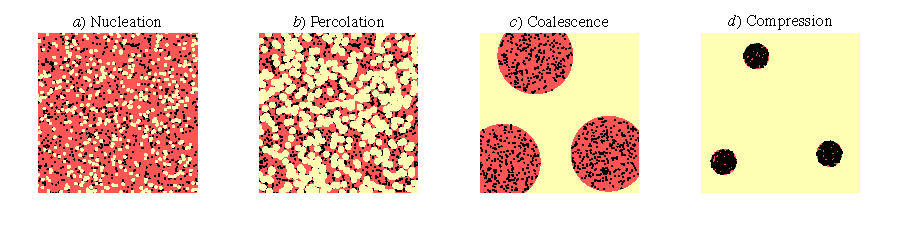
\includegraphics[width=0.98\textwidth]{figs/BolleReviewDM}  \end{center}
\caption[Formation of DM bodies]{\em\label{fig:Bolle} Cartoon of
how a first order phase transition can lead to the compression of DM particles into dense bodies.
Bubbles of the new phase (in yellow) appear and expand.
DM particles, denoted as black dots, cannot enter the new phase and thereby get compressed into remaining small pockets that form after
the bubbles merge.}
\end{figure}


The answer to this question is yes, at least in the weakly coupled models where a DM particle
(either a scalar, fermion or vector) acquires a mass equal to
$m=g w$,  where $w=\langle s\rangle$ is the vacuum expectation value of an extra scalar, $s$, and $g$ is the coupling between DM and $s$~\cite{QballsBis}.
We assume that initially the universe  is in a false vacuum with $s=0$, 
and that it contains relic DM particles with number density $n$ (this could possibly be due to a number asymmetry).
Next, let us assume that $s$  during a first order phase transition at temperature $T  \ll m$ acquires a nonzero vacuum expectation value $s$, and let us denote   
the energy density difference  between the two vacua as $\Delta V$.
During the phase transition, the bubbles of true vacuum with $w\neq 0$ appear, expand, and finally merge. Since inside the bubbles of true vacuum DM particles would have had a large mass $m$, well above the typical thermal kinetic energy of massless DM particles in the false vacuum, energy conservation prevents DM particles from entering the bubbles.
The expansion of bubbles thus compresses DM into small remaining pockets of false vacuum,
as illustrated in fig.\fig{Bolle}.
Each pocket contains a number $Q$ of DM particles, where the statistical distribution of $Q$ values can be computed in any concrete microscopic DM model. 
A variant of this mechanism that leads to microscopic DM candidates has been mentioned in section \ref{bubblecollisionsproduction}.



Of particular interest to us are the models in which {\em i)} the bubble walls move slowly, so that the pockets can dissipate thermal energy, and thus only a small fraction of DM particles escapes via thermal fluctuations, and {\em ii)} the annihilation rate of DM and $\overline{\rm DM}$ particles inside the pockets is negligible (for example, because there is an asymmetry of DM vs $\overline{\rm DM}$ abundances). 
The pockets of trapped DM particles then lead to formation of macroscopic objects.
Compared to the discussion in the previous section, the energy of the system now has additional terms,
\beq \label{eq:UmacroDM}
U = U_{\rm quantum}+ U_{\rm gravity}
 + U_{\rm volume} + U_{\rm surface},
 \eeq
 where
 \beq
 U_{\rm volume}=\Delta V \, \frac{4\pi R^3}{3} ,\qquad
 U_{\rm surface}= \sigma \, 4\pi  R^2,
\eeq
assuming for simplicity a spherical pocket, 
while $U_{\rm quantum}$ and  $U_{\rm gravity}$ are given in eq.~\eqref{eq:Unr} above (in eq.~\eqref{eq:Uquantum:bose} for the bosonic case).
The volume term, $U_{\rm volume}$, is proportional to the potential energy difference $\Delta V$ among the two vacua. Since it scales as $R^3$, it is typically larger than the surface  term due to wall energy density $\sigma$, which only scales as $R^2$, and can thus be neglected for large $Q$.
If the gravitational potential energy is also negligible, then $U \approx  U_{\rm quantum}+ U_{\rm volume}$. 
Since $U_{\rm volume}$ increases with $R$, while $U_{\rm quantum}$ decreases with $R$ (for fixed $Q$), there exists an equilibrium value of $R$.
Its precise value depends on whether DM particles are fermions or bosons due to the different forms of $U_{\rm quantum}$ in the two cases. 
However, in both cases the energy density is constant, $\rho =U/V\sim \Delta V$. That is, in this regime the DM particles trapped inside pockets of false vacua form objects of constant density, just like ordinary matter does, but for a completely different reason --- in this case it is due to a constant energy density difference between false and true vacua, while in solids made out of ordinary matter it is due to almost uniform packing of massive building blocks --- the atoms. 
Having assumed that the DM mass satisfies $m(0) \ll m(s)$, such macroscopic dark bodies have less energy than the free DM quanta would have had, 
if pockets were to be replaced by the true vacuum, and the dark bodies are thereby stable.
DM particles inside the dark bodies are relativistic if $m(0) \ll 1/R$.
On the other hand, if $m(0)$ is big enough so that $U_{\rm gravity}$ is relevant for the stability calculation, 
the macroscopic dark objects can also gravitationally collapse and form either a black hole or a `{\em dark dwarf}'.\footnote{
With the term dark dwarf we denote an object that is physically analogous to a white dwarf 
(normal matter kept together by gravity and quantum pressure),
but made out of dark matter.}

\smallskip

While the above models may seem artificial, engineered such that one ends up with the remnant macroscopic dark bodies, 
the end result may in fact be more generic than one would have naively guessed. 
For instance, a very similar formation history of dark macroscopic objects may occur for
gauge theories with `dark quarks'. 
Assuming, for simplicity, a $\SU(N_{\rm DC})$ gauge dynamics with fermionic dark quarks,
the non-perturbative interactions result in a first order confinement phase transition, 
if the number $N_F$  of fermionic quark flavours lighter than the confinement scale $\Lambda_d$ is either
$3\le N_F \circa{<}3N_{\rm DC}$ or $N_F=0$~\cite{QballsBis}.
In the first case, all the scales relevant for the formation of dark objects are comparable:
$\Delta V \sim\Lambda_{\rm DC}^4$ is comparable to the latent heat, 
the wall pressure is $\sigma\sim\Lambda_{\rm DC}^3$
and the dark hadron masses are of order $\Lambda_{\rm DC}$.
Pockets of false vacuum form with the initial percolation radius smaller than the Hubble length,
$R_{\rm perc}\circa{>} M_{\rm Pl}^{2/3}/\Lambda_{\rm DC}^{5/3}$.
This non-trivial estimate is discussed, e.g.,\ by \href{https://doi.org/10.1103/PhysRevD.30.272}{Witten (1987)} in~\cite{quark:matter:DM} for the case of QCD; see also~\cite{QballsBis}. 
The pockets contain $Q \sim (n R_{\rm perc})^3$ dark quarks, where $n$ is the thermal number density of quarks at the temperature of the phase transition.
Individual dark quarks cannot enter the expanding confined phase (they can only leave the false vacuum pocket, if they form dark baryons in the process), and thus 
get compressed inside pockets until this reach equilibrium radius $R \ll R_{\rm perc}$, where $R$ minimizes eq.\eq{UmacroDM}. 
Only a fraction of dark quarks manage to exit the pockets, 
since a collection of free dark quarks in a false vacuum is lighter than a dark hadron with the same number of constituent dark quarks.
In the same way as the mass of the proton is primarily set by $\Lambda_{\rm QCD}$ rather than by the masses of $u$ and $d$ quarks, 
the mass of the dark hadron is primarily set by $\Lambda_{\rm DC}$.
Macroscopic balls of dark quarks are stable, if they are lighter than the corresponding dark baryons;
in a given theory this depends on the fundamental parameters (such as the dark quark masses) and on the more uncertain 
non-perturbative factors (such as $\Delta V$).
In that case we have, approximately, 
\beq 
Q \sim 10^{23} \, \left(\frac{\rm GeV}{\Lambda_{\rm DC}}\right)^3,\qquad
M \sim \Lambda_{\rm DC} Q\sim {\rm gram} \, \left(\frac{\rm GeV}{\Lambda_{\rm DC}}\right)^2,\qquad 
R\sim \frac{Q^{1/3}}{\Lambda_{\rm DC}} \sim {\rm nm}\,\left(\frac{\rm GeV}{\Lambda_{\rm DC}}\right)^2,
\eeq
for dark quarks that are fermions, while if dark colored particles are bosons one has a somewhat smaller objects, $R\sim Q^{1/4}/\Lambda_{\rm DC}$.
Fig.\fig{MacroCompositeDM} shows the bounds in the  ($M,R$) plane
assuming that dark objects interactions with ordinary matter have cross sections of geometric size. 
Decoupled dark sectors will have smaller cross sections, down to gravitationally small size.

\medskip

A similar discussion applies in the case of no light dark quarks (the $N_f=0$ case). However, in that case also 
an additional, qualitatively different, possibility opens up:
dark quarks can be heavy enough for gravity to 
become relevant in the calculation of properties of macroscopic objects, triggering further gravitational collapse 
of Fermi balls, creating either dark dwarfs or black holes  (for large enough $m$). 


\subsection{Macroscopic objects held together by new forces: $Q$-balls}
\label{sec:Q}
\index{Q-balls}\index{Supersymmetry!Q-balls}\index{DM theory!Q-balls}
In the previous sections we considered macroscopic objects held together by universal forces: gravity, vacuum energy, quantum pressure.
Instead of gravity, a new attractive force could be the reason the macroscopic bodies form.
We bypass lengthy model-dependent discussions and focus on a rather simple case, the $Q$-balls made out of self-interacting scalars whose interactions are described by a fundamendal QFT~\cite{Qballs}. The $Q$-balls themselves are also most easily descried in the language of field theory, where now the amplitude of the scalar field is related to the occupation number, and classical physics emerges when this is large
(the same as the amplitude of the electromagnetic field is related to the number of photons). 
We will thus use the QFT language, at the risk of making $Q$-balls appear to be something deeper than a large number of particles held together by an attractive force. In this language $Q$-balls are described as particular configurations of the scalar  field $\phi$.
In contrast to some other stable field configurations, such as the dark monopoles discussed in section~\ref{Dmonopoles}, 
topology plays no role in the analysis of $Q$-balls and their stability.
The $Q$-balls are simply a bound state of many self-interacting scalar particles, which is
stable because of their binding energy: the $Q$-ball has a smaller total energy than its constituents would have had, had they been free.

\smallskip

The simplest example of a theory in which $Q$-balls can form is a complex scalar field $\phi$ described by a Lagrangian invariant under a global U(1) symmetry, $\phi \to e^{i\delta}\phi$, 
\beq 
\Lag = | \partial_\mu \phi|^2 - V(\phi),\qquad V = m^2 |\phi|^2 +  \lambda |\phi|^4+ \cdots. 
\eeq
Stable $Q$-balls exist if the potential is such that $2V(\phi)/|\phi|^2$ has a local minimum at some field value $\phi_0$, which satisfies
\beq
 \label{eq:QBomega0}
\omega_0^2 \equiv 2 V(\phi_0)/\phi_0^2 < m^2,
\eeq
where $m$ is the mass of a free $\phi$ particle. Above, we have also taken $\phi_0$ to be real, which can always be done without any loss of generality due to the U(1) symmetry.


Spherical field configurations of the form
$\phi = \phi_0 f(r) e^{i \omega t}/\sqrt{2}$
have a global U(1) charge $Q$ and energy $E$ given by
\beq Q = \int dV~i (\phi^*\dot\phi -\phi \dot\phi^*) = \omega \phi_0^2 \int dr\,4\pi r^2 f^2,\qquad
E = \int dr\,  4\pi r^2\,\bigg[ \frac{\phi_0^2}{2} (f^{\prime 2} + \omega^2 f^2) + V\bigg].
\eeq
The profile $f(r)$ is determined by solving the classical equation of motion for field $\phi$, 
$(r^2 f')'/r^2  = \partial V/\partial f/\phi_0^2 -  \omega^2 f$.
One can show that  $dE=\omega\, dQ$: $\omega$ encodes by how much the energy of the $Q$-ball varies when charge is varied.
Generic configurations with a relatively small $Q$ have a smooth profile $f(r)$.
The problem simplifies when $Q$ is large: the solution tends to $f = 1$ inside a sphere of radius $R$
and $f=0$ outside (for details, see \href{https://doi.org/10.1016/0550-3213(86)90520-1}{Coleman (1985)} in \cite{Qballs}). 
In this limiting case the value of $R$ can then be found by minimising $E$, keeping $Q$ fixed, where now
\beq 
Q = \omega \phi_0^2 {\cal V},\qquad E = \bigg[\frac{\omega^2 \phi_0^2}{2}+V(\phi_0) \bigg]{\cal V} ,\qquad
{\cal V} = \frac{4\pi}{3}R^3,
\eeq
and we have already anticipated in the notation that the stable configuration will have constant $\phi$ inside the sphere equal to $\phi=\phi_0$, 
as we now show.
That is, writing $\omega=Q/(\phi_0^2 {\cal V})$  gives $E=Q^2/(2 \phi_0^2 {\cal V})+V(\phi_0){\cal V}$, which, 
when viewed as a function of ${\cal V}$, is minimised for ${\cal V} = Q/\sqrt{2\phi_0^2 V(\phi_0)}$, giving $E = Q\sqrt{2V(\phi_0)}/\phi_0$. 
The energy of the configuration is therefore minimal wherever $2V(\phi)/|\phi|^2$ has a minimum, i.e., at  $\phi_0$ (at which point also $\omega=\omega_0$). Importantly, the value of $\phi_0$ is independent of $Q$, while the energy $E=Q\omega_0$ is directly proportional to the global U(1) charge of the $Q$-ball. 
The $Q$-ball therefore behaves in a similar way as the ordinary matter, where the mass of a block of ordinary material is given by the number of constituents 
(or, equivalently, by the total baryon number). In particular, if one were to emit a single $\phi$ particle from a $Q$-ball, 
its energy would decrease by $\omega_0$, while the free particle at rest at infinity would add energy of its rest mass, $m$, 
so that for $m>\omega_0$ the $Q$-ball is stable. 
 


The minimality condition in eq.\eq{QBomega0} can be satisfied, for example, if $V$ has a local minimum 
away from the origin and $V(\phi_0) >0$. 
So the theory has two minima, a local one at $\phi_0\ne0$, and a global one at $\phi_0=0$. 
This situation is close to (but not yet at) a  first order phase transition, and is an example of an attractive self-interaction,
with eq.\eq{QBomega0} demanding that it is strong enough.
In the limit where the two minima become degenerate, the $Q$-ball volume ${\cal V}$ diverges,
meaning that the system goes through a phase transition.
The $Q$-ball is thus a precursor of the new true vacuum, which after the phase transition encompasses the whole volume. 

\smallskip

In a class of realistic models, the global U(1) can be a baryon or a lepton number,
in which case the existence of $Q$-balls becomes phenomenologically important for the details of baryogenesis.
The scalar $\phi$ could be one of the scalars  present
in supersymmetric models (or, for instance, a linear  combination of scalars that corresponds to a flat-direction in the super-potential); 
then a non-renormalizable term $\sim - |\phi|^6$ is needed 
to satisfy eq.\eq{QBomega0}~\cite{Qballs}.
If U(1) is gauged, the Coulomb potential energy prevents the  existence of $Q$-balls carrying a macroscopically large charge $Q$.
A nontrivial extension of the above discussion is, if the global symmetry is non-Abelian, which can then give rise to more complicated $Q$-balls.

\smallskip


There are several ways in which $Q$-balls can form during the cosmology evolution. If the scalar $\phi$ acquires a large enough vacuum expectation value 
beyond the potential barrier, the field can fragment during later stages of the cosmological evolution, resulting in the formation of $Q$-balls.
Alternatively, first-order phase transitions  can in in some models pack free particles into $Q$-balls,
quite similar to the mechanism discussed in section~\ref{sec:Q2}~\cite{QballsBis}.


\subsection{Axion stars}\label{sec:axionstar}\index{Axion!star}
\index{Stars!axion}
Another example of a macroscopic object whose constituents are possible DM candidates are  {\em axion stars} (also known as {\em boson stars} or {\em Bose stars})~\cite{axion:stars}, which are made out of real scalars.\footnote{For the related case of {\em dark photon stars} (also known as {\em Proca stars}), see~\cite{Procastars}. 
See also \arxivref{1202.5809}{Liebling and Panzula (2012)} in \cite{Procastars} for a comprehensive review of the different bosonic star possibilities. \index{Stars!Proca}\index{Stars!dark photon}\index{Dark photon!star}} 
Perhaps the most celebrated example of such a light scalar is the QCD axion, reviewed in section \ref{axion}, while another is the relaxion, discussed in section \ref{sec:relaxion}. 
More generally, axion stars can be formed by axion-like particles (ALPs, see section \ref{ultralight}), whose interactions with the SM fields are of the same type as those of the QCD axion but whose mass is treated as a free parameter. 
Axion stars are bound state configurations of ALPs, which are stabilised against the collapse 
by a coherent field gradient. 
This makes them distinct from the incoherently oscillating virialized systems such as the axion mini-clusters (section~\ref{AxionCosmo}). 
Since there is no conserved particle number associated with real scalars, axion stars are metastable configurations and eventually decay.\footnote{This is distinct from $Q$-balls, discussed in the previous section, which are made out of complex scalars, and for which there is a conserved quantum number, so that the number of particles, $Q$, is conserved. Due to this conserved charge $Q$-balls cannot decay.} 

\smallskip

There are two distinct branches of possible axion stars, {\em i)} {\em dilute axion stars}, in the formation of which the gravitational potential energy plays an important consideration, and {\em ii)} {\em dense axion stars}, for which gravity is not important. {\bf Dilute axion stars} have 
macroscopically large masses that depend on the number of bound ALPs, $Q$. They cannot grow arbitrarily large, though, since they become structurally unstable above a certain point. 
In this structural instability both gravity and the {\em attractive} force from the tiny ALP quartic negative self-coupling 
$V=m_a^2 a^2/2- (g_4^2/4!) (m_a/f_a)^2 a^4+\cdots$ plays a role~\cite{axion:stars}.
The cosine-like QCD axion potential corresponds to $g_4\sim 0.6$~\cite{axionmodels}. 
Due to very large phase space density of axions, the small interactions can overcome the quantum pressure of eq.\eq{Uquantum:bose},
triggering the collapse of the axion star. 
The energy of an axion star with radius $R$, consisting of $Q$ non-relativistic quanta, can be approximated as
\beq 
U = U_{\rm quantum}+U_{\rm grav} + U_{\rm quartic}\sim \frac{Q}{m_a R^2} - \frac{Q^2 m_a^2}{R M_{\rm Pl}^2}-\frac{g_4^2 Q^2}{f_a^2 R^3}.
\eeq
The first two terms were discussed in eq.s\eq{Uquantum:bose} and \eq{Unr}, respectively. 
The last term estimates the potential energy due to self interactions, $U_{\rm quartic} \sim R^3 V_{\rm quartic}$, in which the amplitude of the axion field $a$ was expressed in terms  
of the number of quanta $Q$ using the relation $Q m_a / R^3\sim m_a^2 a^2$.
Extremising $U$ with respect to $R$ shows that the stable gravitational Bose ball with negligible $U_{\rm quartic}$,
discussed below eq.\eq{Uquantum:bose}, gets destabilised if $U_{\rm quartic}\gtrsim U_{\rm grav}$. This 
implies that axion stars heavier than $ M_{\rm cr }\approx 10 f_a M_{\rm Pl}/m_a g_4$ are unstable.
The order unity numerical factor comes from numerical studies~\cite{axion:stars}.
For the QCD axion with $m_a \approx 10^{-5}\eV$ this critical mass is $M_{\rm cr }\approx 10^{-6}M_\oplus$, and the corresponding radius is $\sim 10^3\km$. 
The radius of an axion star scales as the inverse of the axion star mass, so that lighter dilute axion stars are spatially larger. 

Due to their macroscopic size, the axion stars can have very long lifetimes.  
The microscopic process that leads to the slow decay of an axion star is the $3a\to a$ process, where the final state ALP has enough energy to escape.  The lifetime of a dilute axion star scales roughly as $\tau\propto \exp(1/\Delta_a)$, where $\Delta_a =\sqrt{1-E_a^2/m_a^2}$, with $E_a$ the typical total energy of a single bound ALP (slightly smaller than the rest mass of an ALP, $m_a$), and can thus be stable on cosmological time scales. 
For {\bf dense axion stars} the binding is mainly due to the scalar field potential, with gravity unimportant. 
Typically, they also  have short lifetimes, well below a second, and thus are not objects of interest for cosmology or astrophysics. 

The end results of the axion star collapse depends on the details of the axion couplings. If the coupling to photons is large (about two orders of magnitude larger than in typical QCD axion models) a parametric resonant conversion of axions to photons is reached during growth of axion stars via Bose-Einstein condensation and thus all condensing axions are converted into photons with radio-frequency  $m_a/2$, and an axion star never forms. 
For slightly smaller couplings the parametric resonance is never reached, an axion star forms, 
but during its subsequent collapse the conversion to photons is very efficient and results in a short but powerful burst of radio emissions. 

\smallskip

Let us also recall that very light ALPs, with masses in the fuzzy DM regime, form gravitationally bound solitonic cores at the center of galactic halos, see section \ref{sec:UDM:indirect}.




\section{Origin of Dark Matter stability}
\label{sec:DMSSB}\index{DM properties!stable}
DM needs to be stable on cosmological time scales. 
On the one hand, DM may be absolutely stable, usually due to some symmetry that forbids DM decays. 
Alternatively, DM may be unstable, but with a decay time that is simply much longer than the age of the Universe.
An example of the latter possibility is a sterile neutrino DM, which is 
long-lived thanks to the combination of  a small, keV-scale, mass, 
and the smallness of the mixing angle with the SM neutrinos, that induces the decay, 
see section~\ref{FermionSinglet}. Another example are
primordial black holes, which are long lived because their Hawking radiation is suppressed at large, asteroid-scale, masses. 
Apart from these special cases, theories of DM need mechanisms that highly suppress DM decays.
Broadly speaking these fall into one of the following categories: 
an ad hoc symmetry (section~\ref{sec:adhoc:stabiilty}), 
explicit symmetry present in the theory for other reasons (section~\ref{sec:explicit:stabiilty}), 
or accidental stability (section~\ref{sec:accidentallystable}). 
For a dedicated discussion, see \cite{Hambye:2010zb}.

\subsection{Ad hoc symmetries}\label{sec:adhoc:stabiilty}
The theoretically least appealing possibility is that the DM stability is put in by hand, i.e., by imposing a symmetry that is invoked just to prevent DM decays. The most commonly used symmetries are:
\begin{itemize}
\item[$\blacktriangleright$] {\bf Discrete symmetries.}
The most widely used possibility is the minimal one: a $\mathbb{Z}_2$ symmetry under which DM is odd, while any lighter particles are even, thus preventing DM to decay.
Some DM models, though, rely on $\mathbb{Z}_3$ or higher $\mathbb{Z}_N$ symmetries for DM stability. 
\item[$\blacktriangleright$]
{\bf Global symmetries. }The simplest and also the most commonly used possibility is a global dark U(1) under which DM particles carry a nonzero charge.
It implies a conservation of the associated DM number, and also allows for cosmological evolutions that lead to a non-zero DM asymmetry.
\end{itemize}
Gravity is expected to break global symmetries, both continuous and discrete.
However the numerical size of the effect is unknown, and could be negligible for any practical purpose
(in the same way as the baryon number in the SM is not exactly conserved, 
and is broken by sphaleron field configurations that are completely negligible at low temperatures).



\subsection{Symmetries motivated by other reasons} \label{sec:explicit:stabiilty}
The symmetry that guarantees the stability of DM could be a consequence of a bigger symmetry structure
within a full theory, which apart from DM particle and the SM contains also other states. 
 \begin{itemize}
 \item[$\blacktriangleright$] {\bf Supersymmetric} models such as the MSSM assume a  $\mathbb{Z}_2$  symmetry, $R$-parity,
 under which all the supersymmetric particles are odd and all the SM particles are even. The $R$-parity was introduced in order
 to avoid phenomenological problems: 
 to ensure sufficient proton stability and to weaken bounds on new flavour-violating effects,
 see section~\ref{SUSY} for further details. 
A side implication is that the lightest supersymmetric particle is stable and can thus be a DM candidate. 

 \item[$\blacktriangleright$] 
Some of the possible dark gauge groups predict extended field configurations that are stable for {\bf topological reasons}, 
and could thus be DM candidates. For instance, dark magnetic monopoles are stable for topological reasons in theories
where a gauge group $\mathcal{G}$ is spontaneously broken to a sub-group $\mathcal{H}$,  where
$\mathcal{H}$ contains U(1) factors (section~\ref{Dmonopoles}).


\item[$\blacktriangleright$] {\em If} {\bf something different} than the usual fermions and bosons can make sense within QFT, 
this something might only couple in pairs to the rest of the SM, and thereby be a stable DM candidate.
Possible speculative ideas along these lines are: 
\begin{itemize}
\item[$\rhd$] DM as a para-fermion (a tentative particle with intermediate quantum statistics)~\cite{1807.07289}.
\item[$\rhd$] DM as a dimension-1 `{Elko}' fermion, which is a non-local representation of the Lorentz sub-group spanned by the
$J_z$, $K_z$, $K_x+J_y$, $K_y-J_x$ generators. 
The fact that it contains all $K_{x,y,z}$ boosts avoids the strongest bounds on Lorentz violation~\cite{1008.0436}.

\item[$\rhd$] \href{https://doi.org/doi:10.1098/rspa.1971.0077}{In 1971 Dirac} proposed 
a system of relativistic particles with mass $M$ and positive frequency only, described by
an infinite-component wave equation~\cite{Dirac71}.
This system of particles only (without anti-particles) received little interest because it cannot be consistently coupled to gauge fields, and also other SM fields.
This property becomes favourable for a DM candidate~\cite{Dirac71}. 

\item[$\rhd$] 
Gauge-invariant QFT are usually restricted to quantum states on which expectation values satisfy
the classical equations of motion, such as the 1st Maxwell equation (in electromagnetism)
and/or the 1st Friedmann equation (in general relativity).
More general quantum states violate such classical equations, by containing electric or gravitational fields as those
generated by extra stable charge and/or mass, despite that such sources are not present.
This phenomenon can be identified as DM, up to the problem that cosmological inflation would dilute it~\cite{Rajendran24}.
\end{itemize}
\item[$\blacktriangleright$]  
{\bf Symmetry breaking} can leave a residual symmetry that protects DM stability.
\begin{itemize}
\item[$\rhd$] 
A simple possibility, which requires at least two matter fields extending the SM, is that DM carries a charge $+1$ under a  dark $U(1)_d$ gauge group, which is spontaneously broken by a vacuum expectation value of a scalar with dark charge $+2.$ 
This then leaves a $\mathbb{Z}_2$ subgroup of $U(1)_d$ unbroken.
This kind of structure can arise from bigger groups that admit spinorial representations.

\item[$\rhd$]
The SM motivated $\U(1)_{B-L}$ group can lead to DM candidates, assuming suitable fractional charges~\cite{1509.04036}.

\item[$\rhd$] The residual symmetry protecting DM stability can also occur in extensions of the SM by a single field. Such theories with a minimal field content can even be systematically classified.
That is, a dark gauge group (SU$(N)$, SO$(N)$, ${\rm Sp}(N)$ or exceptional groups)
broken spontaneously to a sub-group $\mathcal{H}$ by a single scalar $S$ in a given representation
sometimes results in acceptable DM candidates~\cite{VectorDM}.
These theories have only a few free parameters, and predict a non-trivial cosmology and phenomenology. 
For instance,  $\mathcal{H}$ can confine at energies below the spontaneous symmetry breaking scale, which can result in a composite DM.
In some cases such DM candidates are stable at the renormalizable level, and the symmetries ensuring its stability are of accidental nature.
This is discussed  in section~\ref{sec:accidentallystable}, together with the non-trivial mathematics of Lie groups.
\end{itemize}

\end{itemize}


\subsection{Accidentally stable Dark Matter}\label{sec:accidentallystable}
An interesting possibility is that DM stability is due to an accidental symmetry,
analogous to how the accidental baryon number explains the proton's quasi-stability in the SM 
(baryon number conservation in the renormalizable SM Lagrangian arises simply as a consequence of the assumed field content and gauge symmetries).
A variety of accidental symmetries can similarly lead to a stable DM candidate:
\begin{itemize}
\item[$\blacktriangleright$] DM might be a {\bf fermionic 5-plet} under weak $\SU(2)_L$, as discussed in section~\ref{MDM}. 

\item[$\blacktriangleright$] 
DM might be stable due to an accidental symmetry in a dark sector.
For example, DM might be analogous to the proton:
a composite particle under a new confining gauge group,
stable thanks to an accidental U(1) {\bf dark baryon number}. 
Another related possibility is that DM is a dark pion stable thanks to a dark flavour symmetry or due to dark $G$-parity,
as discussed in section~\ref{sec:compositeDM}.


 \item[$\blacktriangleright$] 
 DM stability could also be due to more profound versions of accidental symmetries of a group theoretical nature in the dark sector, for instance, due to automorphisms
that some of the gauge groups admit.
The simplest example of an automorphism is  {\bf charge conjugation}, for which the simplest realization 
is DM that is a dark U(1) gauge boson $A_\mu$, 
 which obtains its mass after a  scalar $S$ charged under the dark U(1) acquires a vacuum expectation value.
Despite the symmetry breaking, the massive dark gauge boson remains stable, 
if the theory is invariant under charge conjugation in the dark sector, 
\beq S\to S^*,\qquad A_\mu\to - A_\mu.\eeq
In this simple model, charge conjugation  is, however, not an accidental symmetry, because it
can be broken by the kinetic mixing between hypercharge and dark U(1)~\cite{VectorDM}.
Therefore an abelian vector $A_\mu$ is a viable DM candidate only if this mixing is sufficiently suppressed.

\item[$\blacktriangleright$] 
A less minimal example is that DM particles are the three gauge bosons of an $\SU(2) $ dark gauge group that is 
completely spontaneously broken by a scalar $S$ in the fundamental representation 2 of SU(2) 
that obtains a non-zero vacuum expectation value.
The three $\SU(2)$ vectors are stable DM candidates~\cite{VectorDM} 
because the theory is accidentally invariant under the {\em charge conjugation
in the dark sector}, 
\beq S\to S^*, \qquad A_\mu^a T^a \to -(A_\mu^a T^a)^*,\eeq 
where $T^a$,  $a=\{1,2,3\}$, are the gauge group generators in the fundamental representation.
The CP-odd stable vectors are associated with the real $T^a$ generators of the fundamental representation,
namely the $T^{1,3}$ generators, in the usual notation.
This theory also contains a larger accidental custodial global  symmetry, 
such that the three vectors acquire a common mass $M$.
The dark topological term, $A_{\mu\nu}^a\tilde A^{a\mu\nu}$, gives exponentially small CP-violating contributions for small values of gauge coupling.

More generally, complex conjugation is a non-trivial
$\mathbb{Z}_2$ outer automorphism of the $\SU(N)$, $\SO(2N)$ and $E_6$ groups
with symmetric Dynkin diagrams.
So the accidental DM stability of the type discussed above can be realized in many different contexts.


\item[$\blacktriangleright$]
Some DM theories with a dark gauge group
can be accidentally invariant under a $\mathbb{Z}_2$
discrete symmetry, which acts on components of dark multiplets rather than on full multiplets. An example is a $\mathbb{Z}_2$ under which
only the $i=1$ component of a field in the fundamental representation of the symmetry group is odd, 
while the remaining components are $\mathbb{Z}_2$ even. For other representations, the transformation rules can be built by considering products of fundamentals. 
For instance, dark vectors can be written as a matrix $(A^a T^a)_i{}^j$, and the $i=j=1$ indices are taken to be odd.
This symmetry is called {\bf group parity} because it is analogous to space-time parity,
except that it acts in group space.
In a theory with an unbroken group parity, the lightest parity-odd state is stable.
For instance, group parity can ensure the stability, for any $N$, of  the $\SO(N)_{\rm DC}$ baryons, 
which are states built by contracting dark fermion fields $\Psi_i$ with the anti-symmetric tensor.

\item[$\blacktriangleright$] Special groups with symmetric Dynkin diagrams contain extra special symmetries that can also ensure DM stability:
SO(8) contains a {\bf triality}; the  exceptional group $\mathcal{G}_2$ an  inner automorphism
(see, e.g.,~\arxivref{1911.04502}{Buttazzo et al.} in~\cite{VectorDM}), etc. 
\end{itemize}
 

